% !TEX root = ../IS.tex
\chapter{Description of Software}
\section{AI Model}
\subsection{Simulation Model}
For this thesis, a 2D, turn-based role-playing game (RPG) was created, titled \textit{Cave Escape}. In an RPG, players are given a list of possible actions they may take on their turn. These actions consist of, but are not limited to: attacking (usually with a melee weapon), using magical spells (of both offensive and defensive varieties), and using items (to either heal players or otherwise make them more powerful). These choices are tied to the character the player controls, along with their character stats. A thief character may be faster and more nimble, but may also be weaker and unable to use magical spells. A knight character could be stronger and better defended with their armor, but also slower and easier for opponents to hit. With regards to player actions and choices, the thief may be able to steal items, while the knight may be able to block attacks with a shield. This is the ``role-playing'' aspect of the game: the player chooses their actions based on the role of their in-game character.\\

\begin{figure}[H]
  \centering
  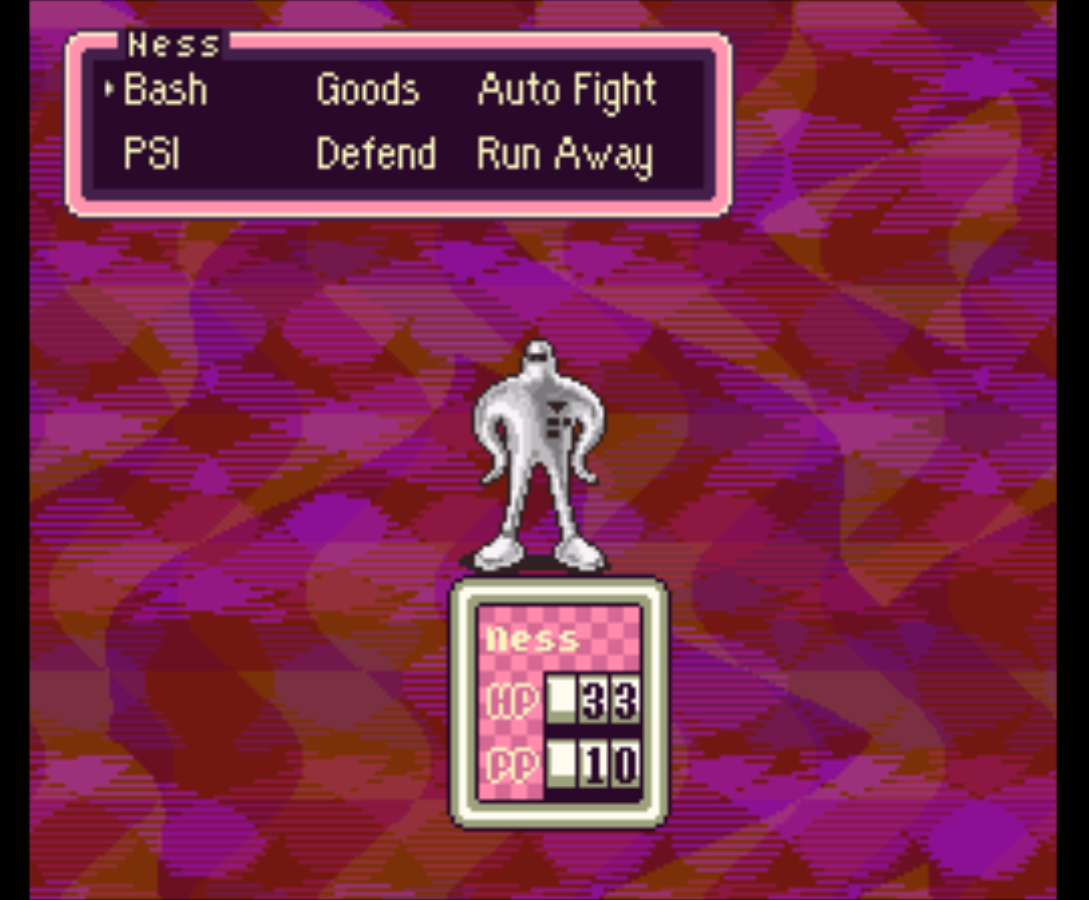
\includegraphics[width=9cm]{figures/Earthbound.png}
  \caption{A screenshot of a battle from the turn-based role-playing game \textit{Earthbound} \cite{earthbound94}.}
  \label{fig:Earthbound}
\end{figure}

For instance, observe the battle shown in Figure \ref{fig:Earthbound} from the game \textit{Earthbound}. The computer opponent is shown in the center of the screen. At the top, the actions available to the player are listed. Players have the choice of making a melee attack (Bash), casting a magical spell (PSI), using an item (Goodies), or reducing damage taken (Defend). Players can also select Auto Fight to have the computer make all the choices for them, or they can Run Away and escape from the battle. At the bottom, the hit points (HP) and psychic points (PP) of the character are shown - these correspond to the character's health and their magical abilities.

Specific to turn-based RPGs, the player has as much time as they want to decide on their strategy. This is in contrast to an action RPG, where combat takes place in real-time. Generally, action RPGs use 3D environments to better accommodate the real-time battles, but this is not always the case. In the game created for this thesis, a turn-based approach is better suited because it emphasizes player strategy. Action RPGs may have similar lists of commands and actions, but these actions frequently have a corresponding skill component.\\

Take for example a basic attack. In a turn-based RPG, this action requires little from the player: they select that choice from a list, and their in-game character attacks the opposing player. Depending on the game, this attack may or may not be successful - the opponent could dodge or block the hit - but the success or failure is determined by the game through the stats both players - if for instance a character is nimble enough to dodge, or defensive enough to block a strike. An action RPG, on the other hand, determines whether an attack misses or hits through hit-boxes. A hit-box is a hidden area tied to some in-game object; when hit-boxes intersect, something happens depending on the types of objects. For this example, an attack would be successful if the hit-box of the character's attack (their sword, fist, magic spell, etc.) intersects with the hit-box of their opponent's body. The attack would fail if these hit-boxes do not intersect. Thus, the overall success of a character in an action RPG is dependent on a player's skill in making hit-boxes collide. This type of gameplay does not lend itself well to game theory analysis, as a player could make all the right decisions but still lose from lack of skill.\\

\begin{figure}[H]
  \centering
  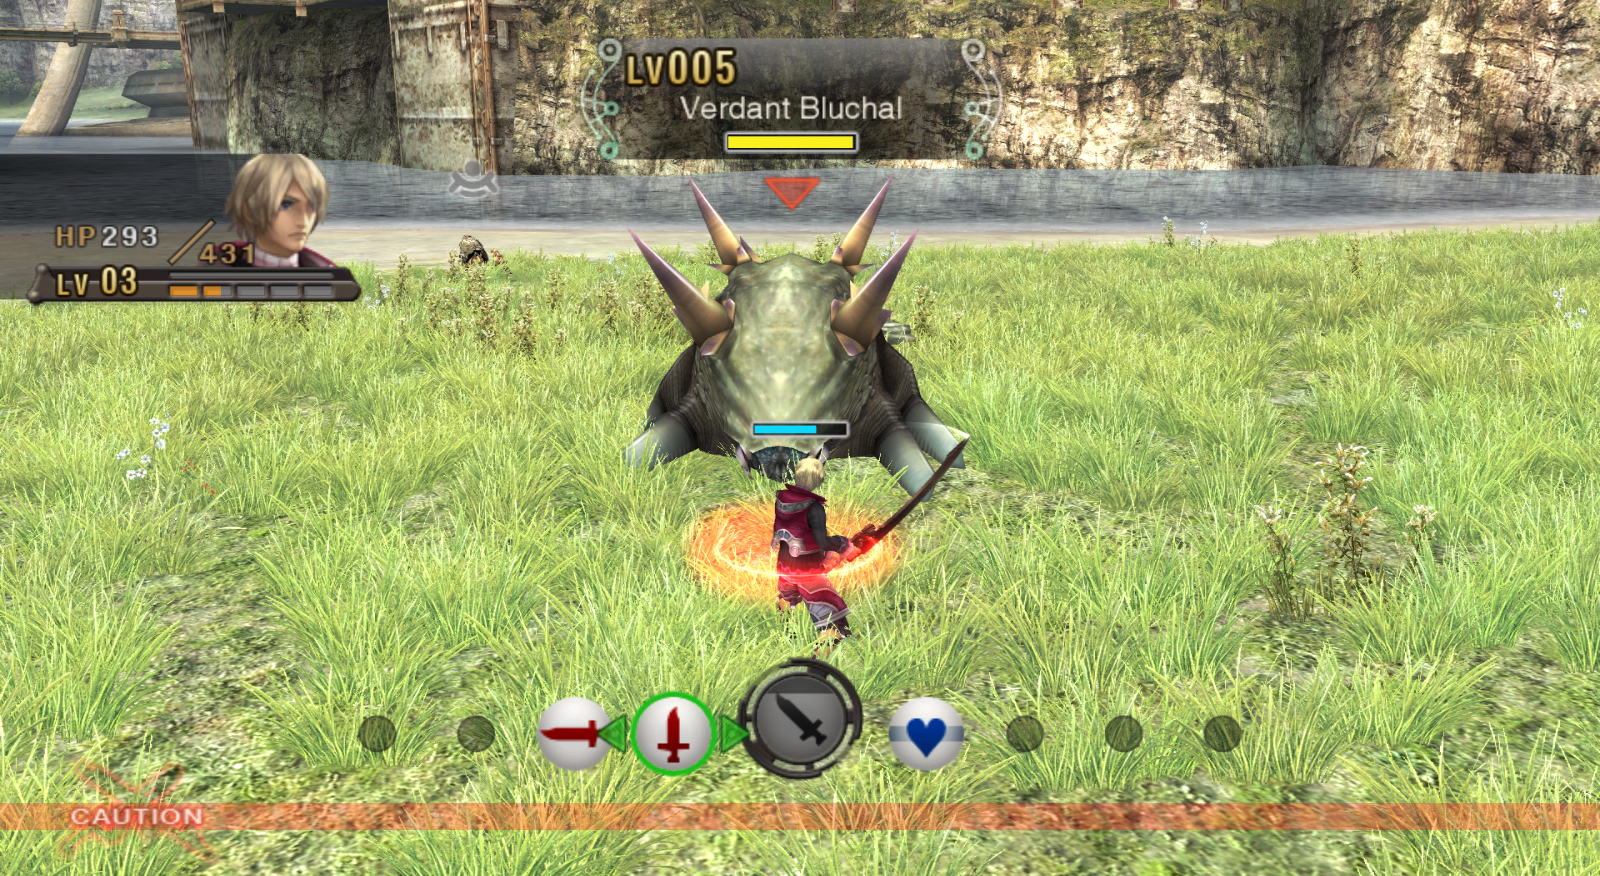
\includegraphics[width=9cm]{figures/Xenoblade.png}
  \caption{A screenshot of a battle from the action role-playing game \textit{Xenoblade Chronicles} \cite{xenoblade10}.}
  \label{fig:Xenoblade}
\end{figure}

For more a concrete example, regard a battle from the action RPG \textit{Xenoblade Chronicles}, as shown in Figure \ref{fig:Xenoblade}. In this game, the player can move freely in 3D space. The character shown has four abilities, represented as icons along the bottom of the screen. The two red-tinted abilities are attacks, as is the shaded center ability. The blue ability on the right is a healing spell. The skill component of this game comes with the two red abilities; these abilities do more damage and cause additional affects when performed at certain angles. For instance, the leftmost ability does more damage when used on an opponent's side, while the second red ability does more damage when used from an opponent's back. Thus, two players could use the same series of abilities but have different outcomes based on how their attacks were positioned.\\

Similarly, the game presented in this thesis is a two-dimensional game. With a turn-based RPG, since the gameplay involves choosing actions from a list, the only difference between a 2D and a 3D turn-based RPG is the graphical quality. A 2D game uses sprites, while 3D games use polygonal models. A two-dimensional game was chosen to simplify development.\\

To begin building an AI model, we first create a simulation of the \textit{Cave Escape}. The simulation has two players, each with 25 health points (HP). In this first simulation, both players have two possible actions per turn which are randomly selected: attack the other player, reducing their opponents HP by 5 points, or heal themselves, increasing their HP by 4 points. Players can not heal above their starting value of 25 HP; any extra health points are discarded. Each action has a 50\% chance of occurring. The game runs until one player's HP is reduced to 0. The total number of turns and the sequence of actions are recorded into a CSV file. After running 4500 simulations, the data is imported into Matlab. A subset of the games are used as a training set for a decision tree, which predicts the player that wins the game.\\

\begin{figure}[H]
  \centering
  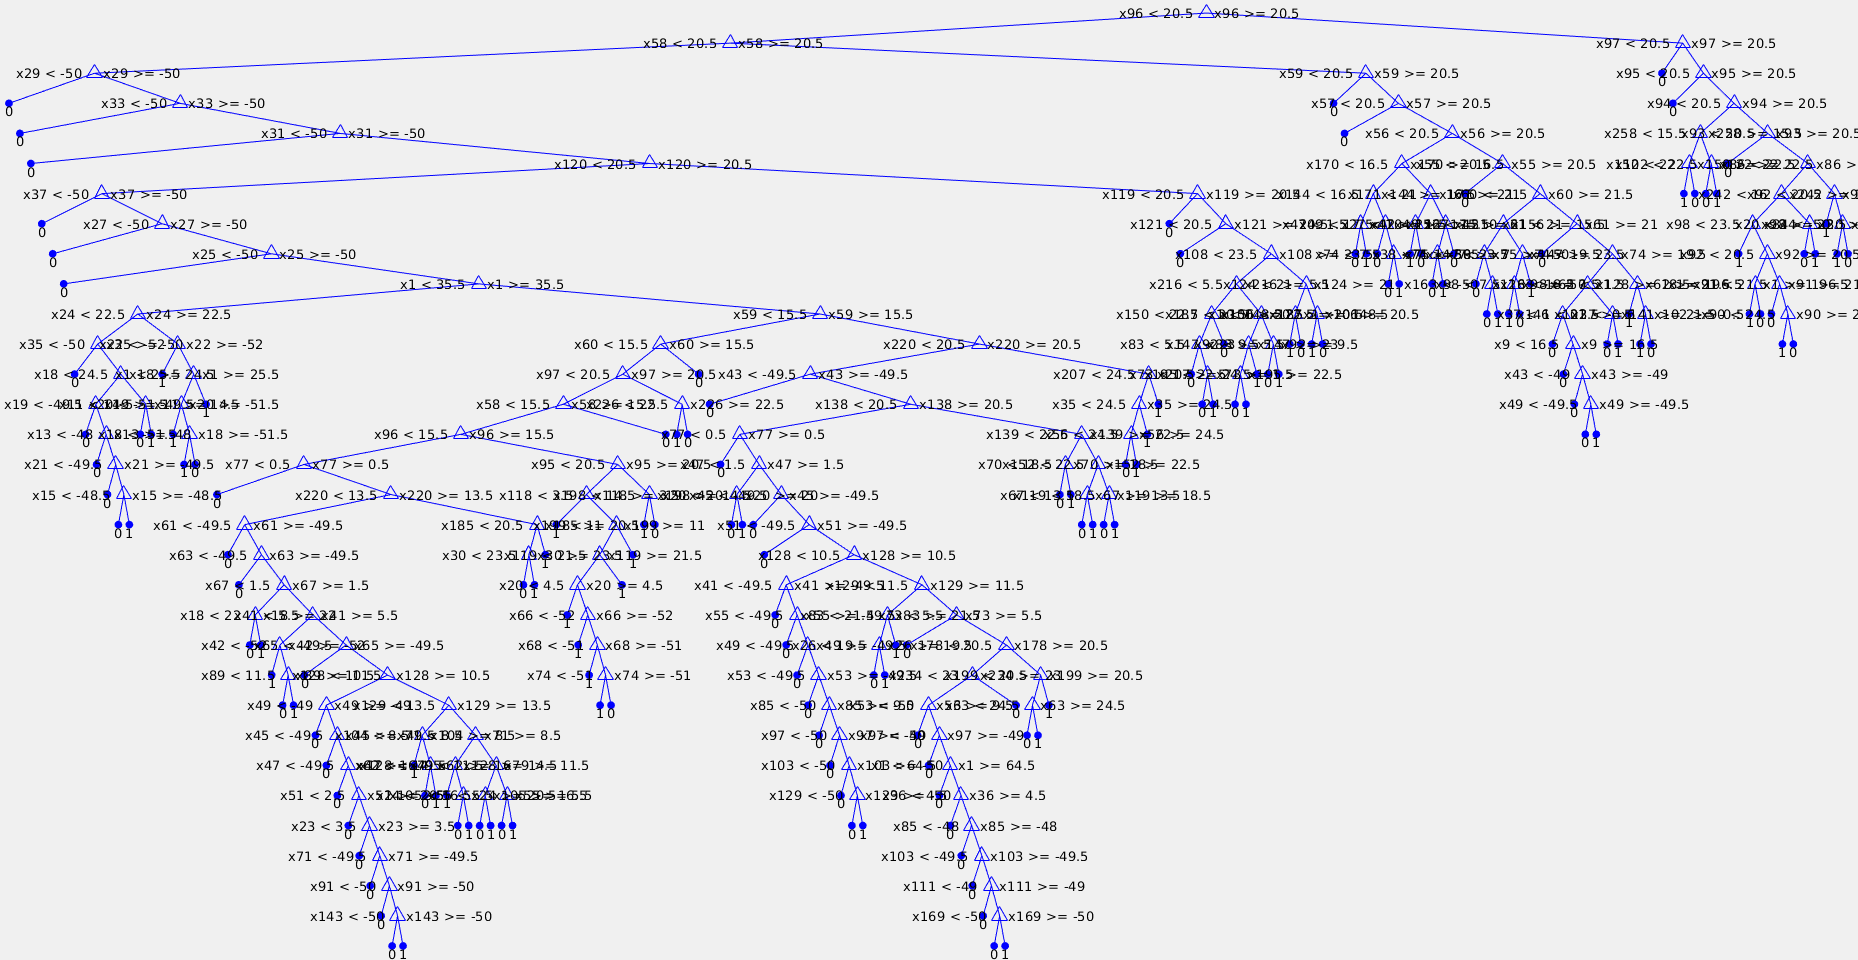
\includegraphics[width=13cm]{figures/firstDecisionTree.png}
  \caption{The decision tree generated from 4000 simulations of the game. This tree predicts 0 when player 1 wins and 1 when player 2 wins.}
  \label{fig:decisionTree1}
\end{figure}

However, this method is inconclusive, for a number of reasons. Firstly, the decision tree includes a  large number of branches, as seen in Figure \ref{fig:decisionTree1}. Secondly, the actual criteria evaluated at each branch of the tree is different for each game. Aside from the first column, which contains the total number of turns in the game, and the second column, which contains the starting HP of player 1, the values in any particular column differ from game to game. For instance, the root node uses the value in column 96 as its classifier. In one game, column 96 may contain a HP value for player 2. In another, longer game, that column may contain a HP value for player 1. Thirdly, the individual games contain numerous streaks: a longer game is not the result of better strategy, but is instead caused by streaks where both players choose to heal on their turns. Players in these streaks reach HP levels near the 25 HP cap, effectively resetting the game.

The lack of consistency along columns is most likely the largest detriment to this model. Decision trees work best when classifying problems on specific attributes; if the attribute is different at column 96 from one game to another, the information gain at that column is meaningless. This is likely behind the sprawling nature of the decision tree itself. Without clear attributes to test, each split only has minuscule amounts of information gain.

\subsection{Extensive Tree Model}
A game theoretic angle is used on the second attempt. The HP of both players is reduced to 10, and two restrictions are added on healing: a player can not heal when they have full health, and a player can only heal themselves twice. As in the first attempt, players can only attack or heal. With these new rules in place, we create an extensive-form tree for the new game.\\

\begin{figure}[H]
  \centering
  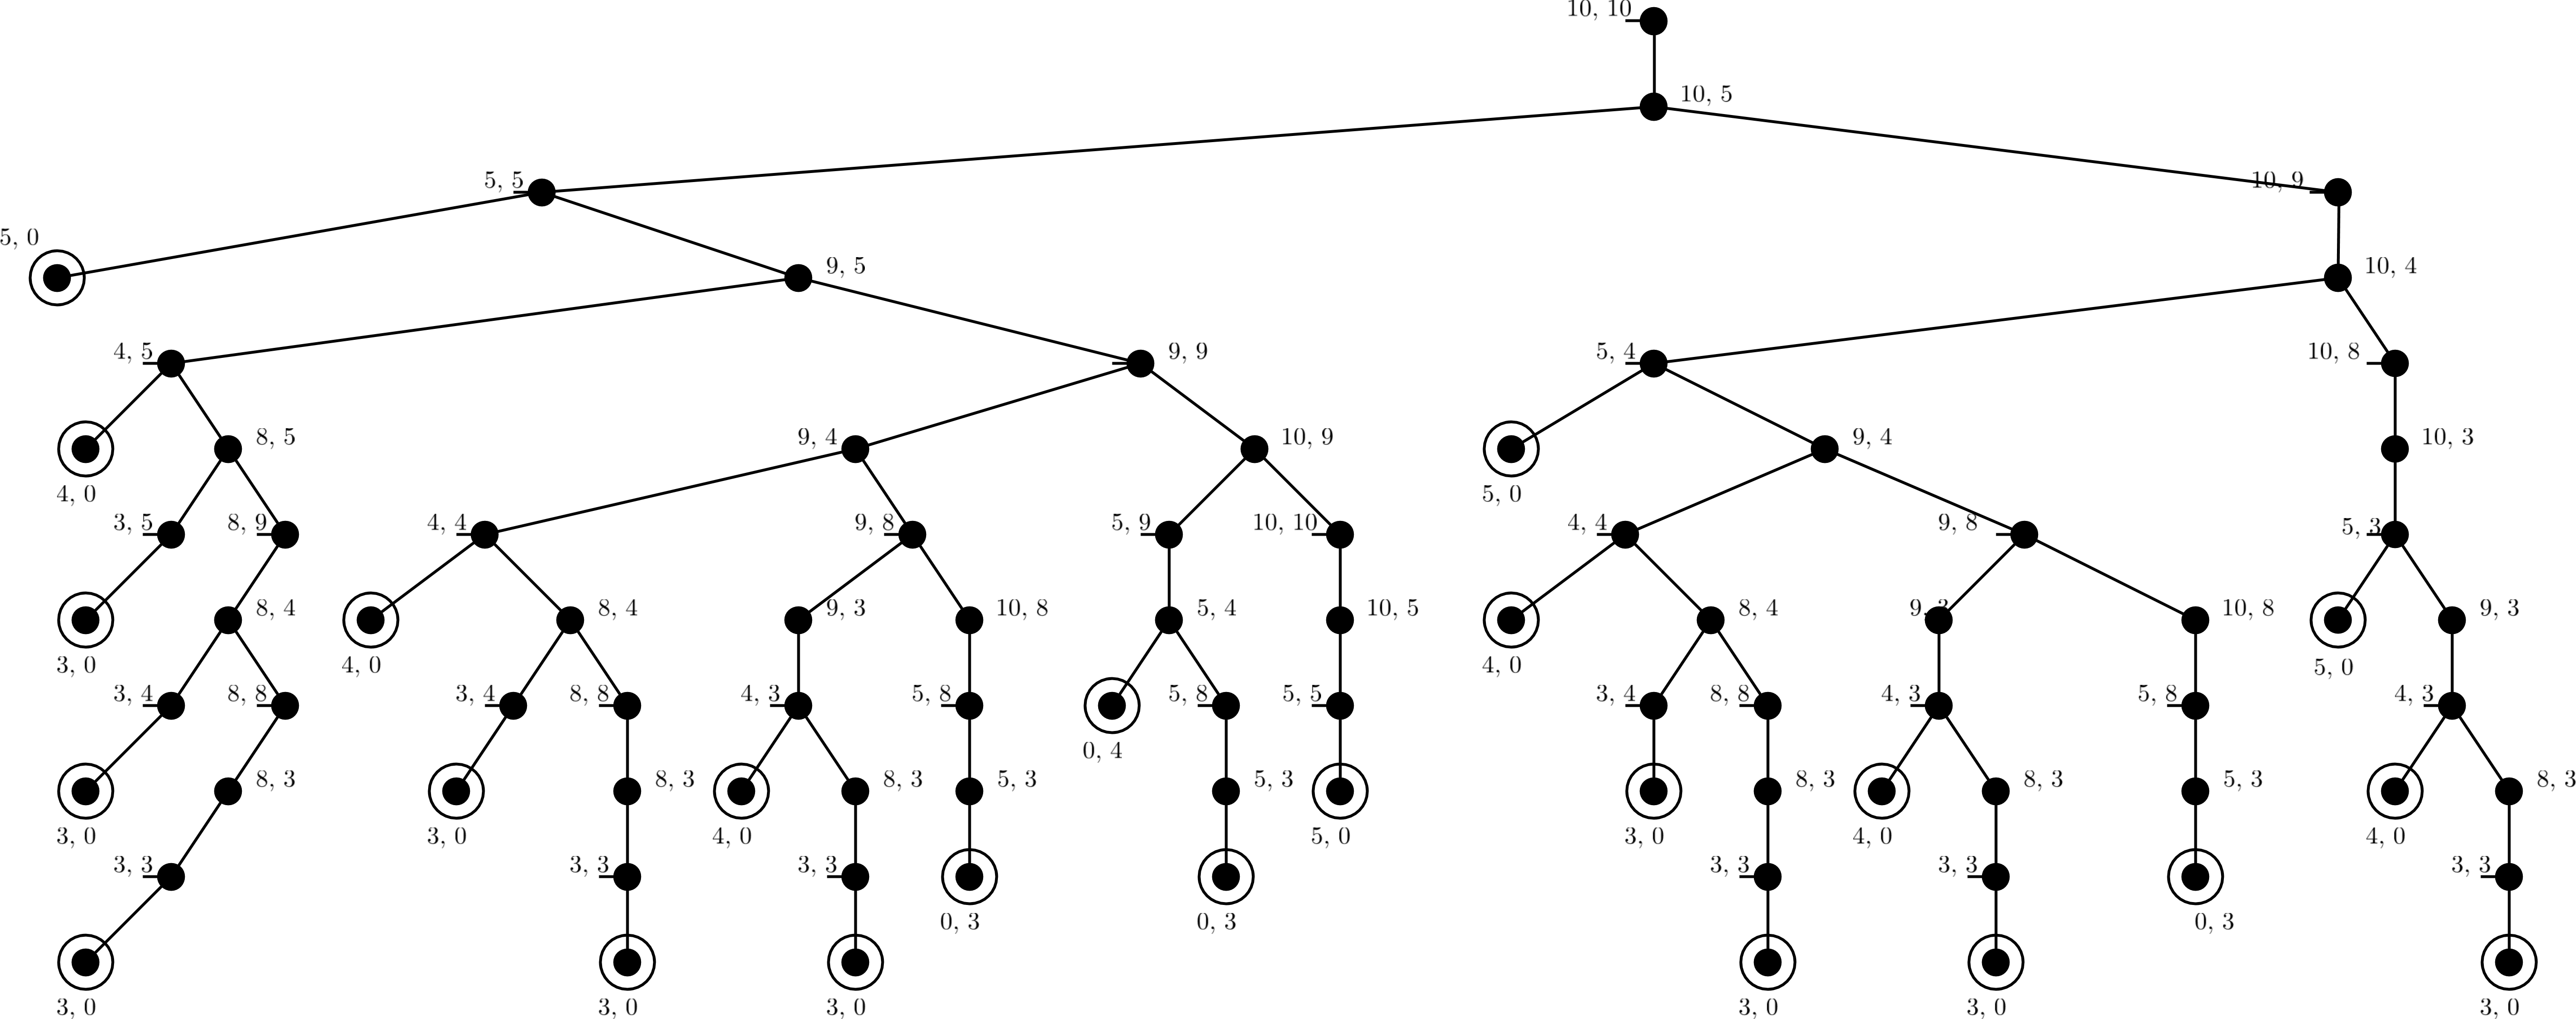
\includegraphics[width=15cm]{figures/GameTree.png}
  \caption{The extensive-form tree for a simplified game. Each player starts with 10 hit points (HP). At each node, a player can choose to heal themselves or attack their opponent. Attacking reduces the opponent's HP by 5 points. Healing increases the decision maker's HP by 4 points; they can only heal themselves twice per game.}
  \label{fig:gameTree}
\end{figure}

In Figure \ref{fig:gameTree}, player 1's nodes are denoted by a small dash to the left of the node. The HP values of both players are recorded at each node. Leaf nodes where player 1 wins are enclosed in a circle, and leaf nodes where player 2 wins are enclosed in a diamond. There are 24 outcomes for this game; of these, only 4 of them result in a win for player 2, while the other 20 result in wins for player 1. In fact, with optimal play, player 1 always wins in this game.\\

\begin{figure}[H]
  \centering
  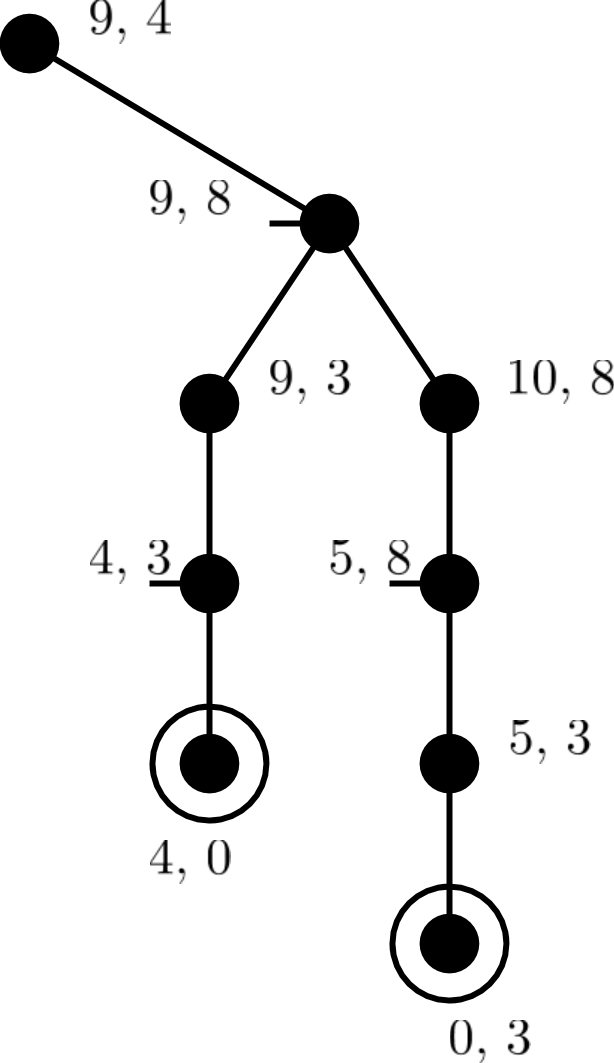
\includegraphics[width=4cm]{figures/GameSubtree.png}
  \caption{A subtree of the extensive-form representation in Figure \ref{fig:gameTree}. This subtree contains one of player 2's only winning outcomes.}
  \label{fig:gameSubtree}
\end{figure}

For example, in the subtree shown in Figure \ref{fig:gameSubtree}, both player 1 and 2 have a winning outcome. However, the critical decision is made by player 1. If player 1 chooses to heal, then player 2 will win in 3 more turns. If player 1 chooses to attack, then player 1 will eventually win. Thus, in any game which reaches this subtree, player 1 chooses to attack on their turn, since that choice leads to their victory.\\

\begin{figure}[H]
  \centering
  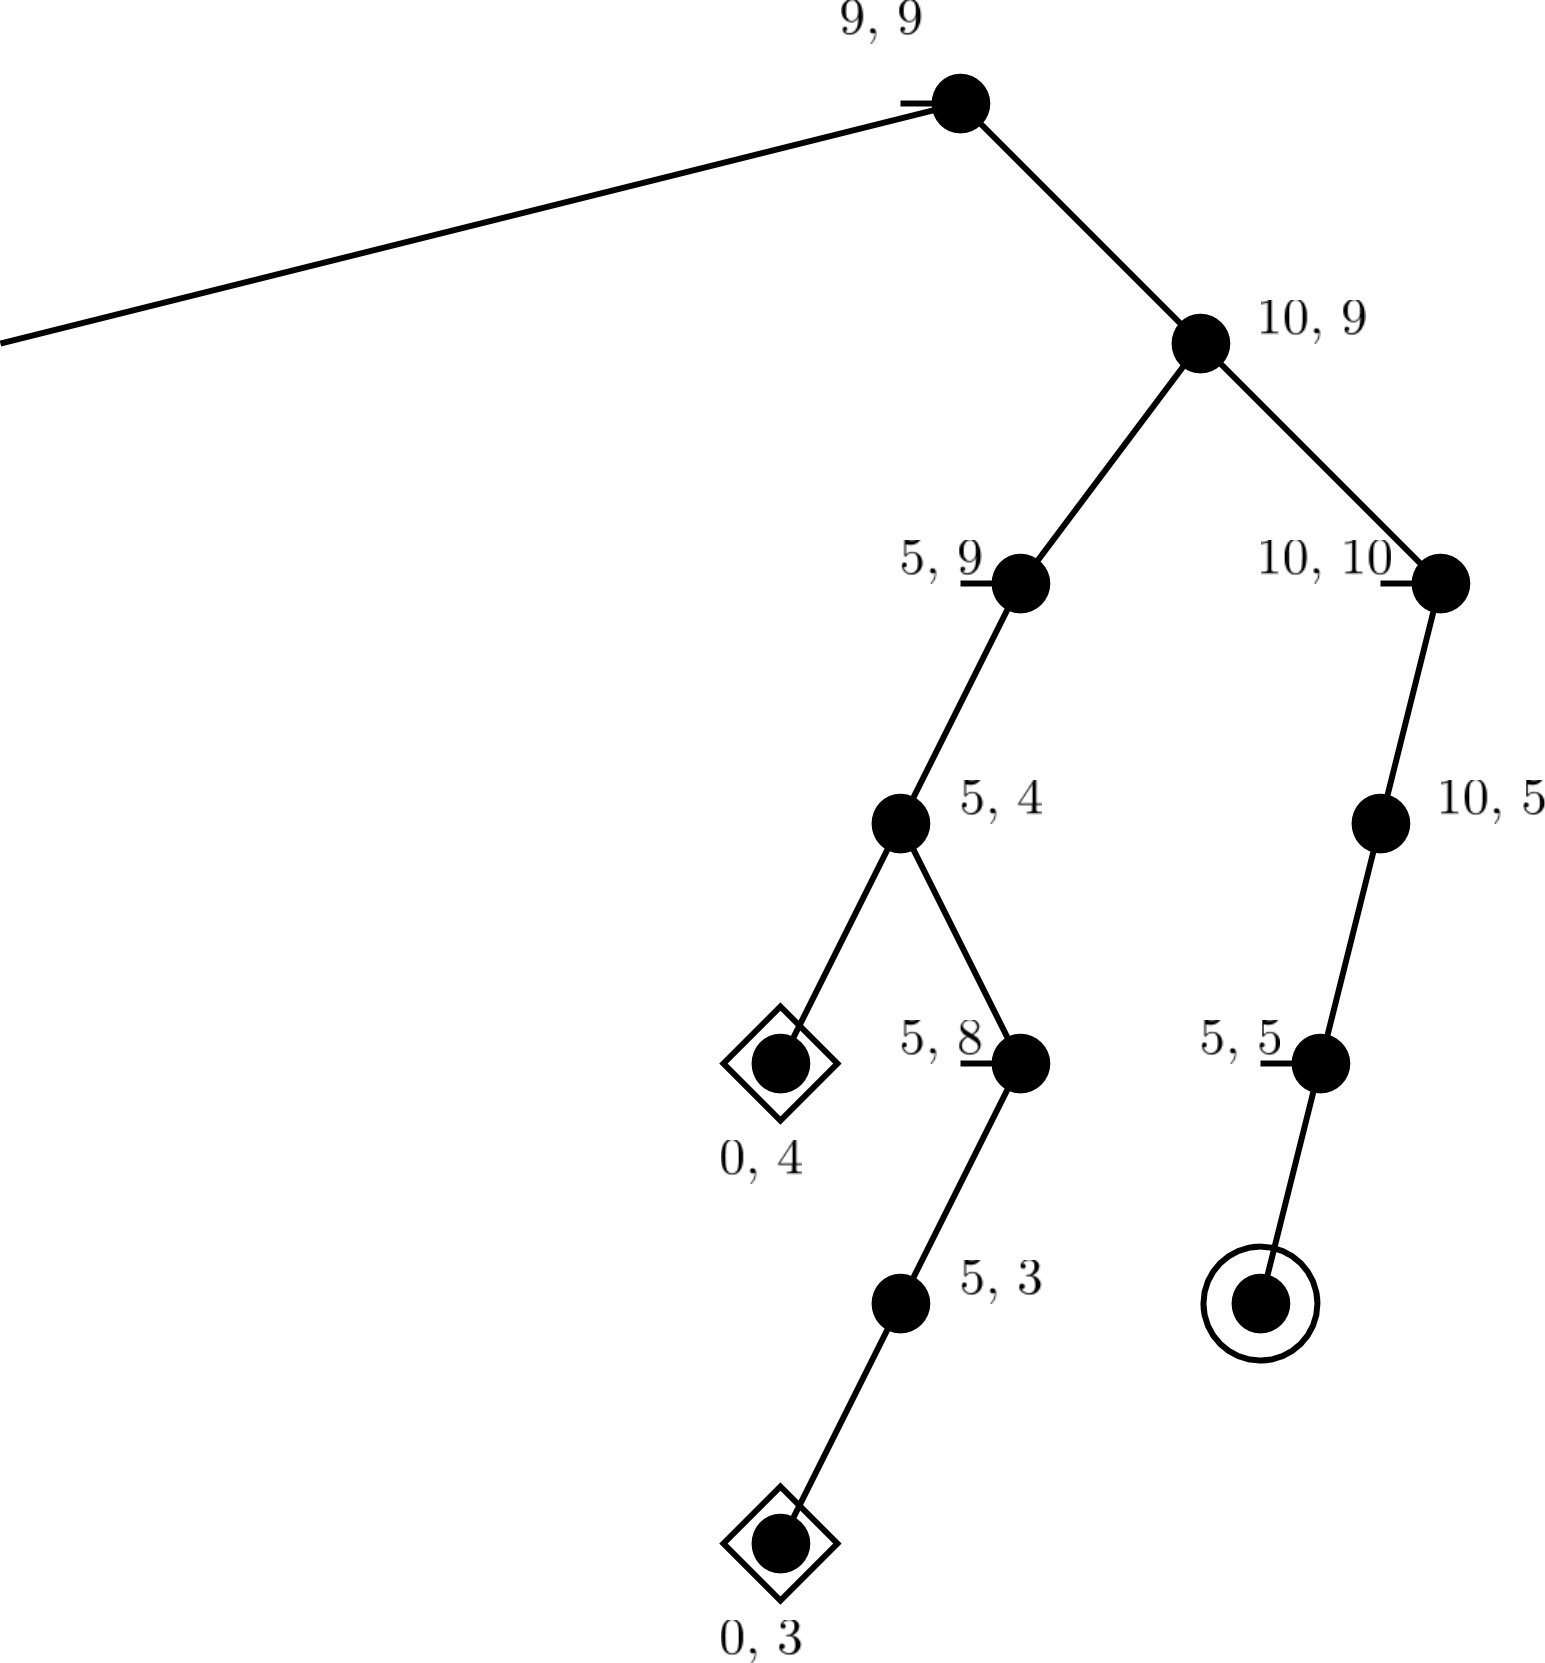
\includegraphics[width=8cm]{figures/GameSubtree2.png}
  \caption{A second subtree of the extensive-form representation in Figure \ref{fig:gameTree}. This subtree contains two more of player 2's winning outcomes.}
  \label{fig:gameSubtree2}
\end{figure}

Two more of player 2's winning outcomes can be seen in the subtree in Figure \ref{fig:gameSubtree2}. At the root node of this subtree, player 1 is making their choice. If they choose to heal, the game moves into the right child. Player 2's first choice on the right child's subtree either results in a win (if player 2 attacks) or a loss (if player 2 heals). Thus, an intelligent player 2 would always attack at this stage, since it is a guaranteed win. However, if player 1 knows that this is a guaranteed win for their opponent, player 1 can avoid this threat by attacking instead of healing at the root node.\\

If player 1 decides to avoid the subtree in Figure \ref{fig:gameSubtree2}, player 2 has the next choice. If player 2 decides to heal at this new node, then the resulting subtree is identical to the one found in Figure \ref{fig:gameSubtree}. This subtree contains player 2's final winning outcome, but once again player 1 can avoid this outcome with ease.\\

\subsubsection{Backwards Induction on Extensive Tree Model}
We can prove that player 1 will always win this game through the backwards induction algorithm discussed in Chapter 2. Recall that the algorithm travels through a game tree by recursion and, at each node, returns the child node which gives the player acting at the parent node the most utility.

\begin{figure}[H]
  \centering
  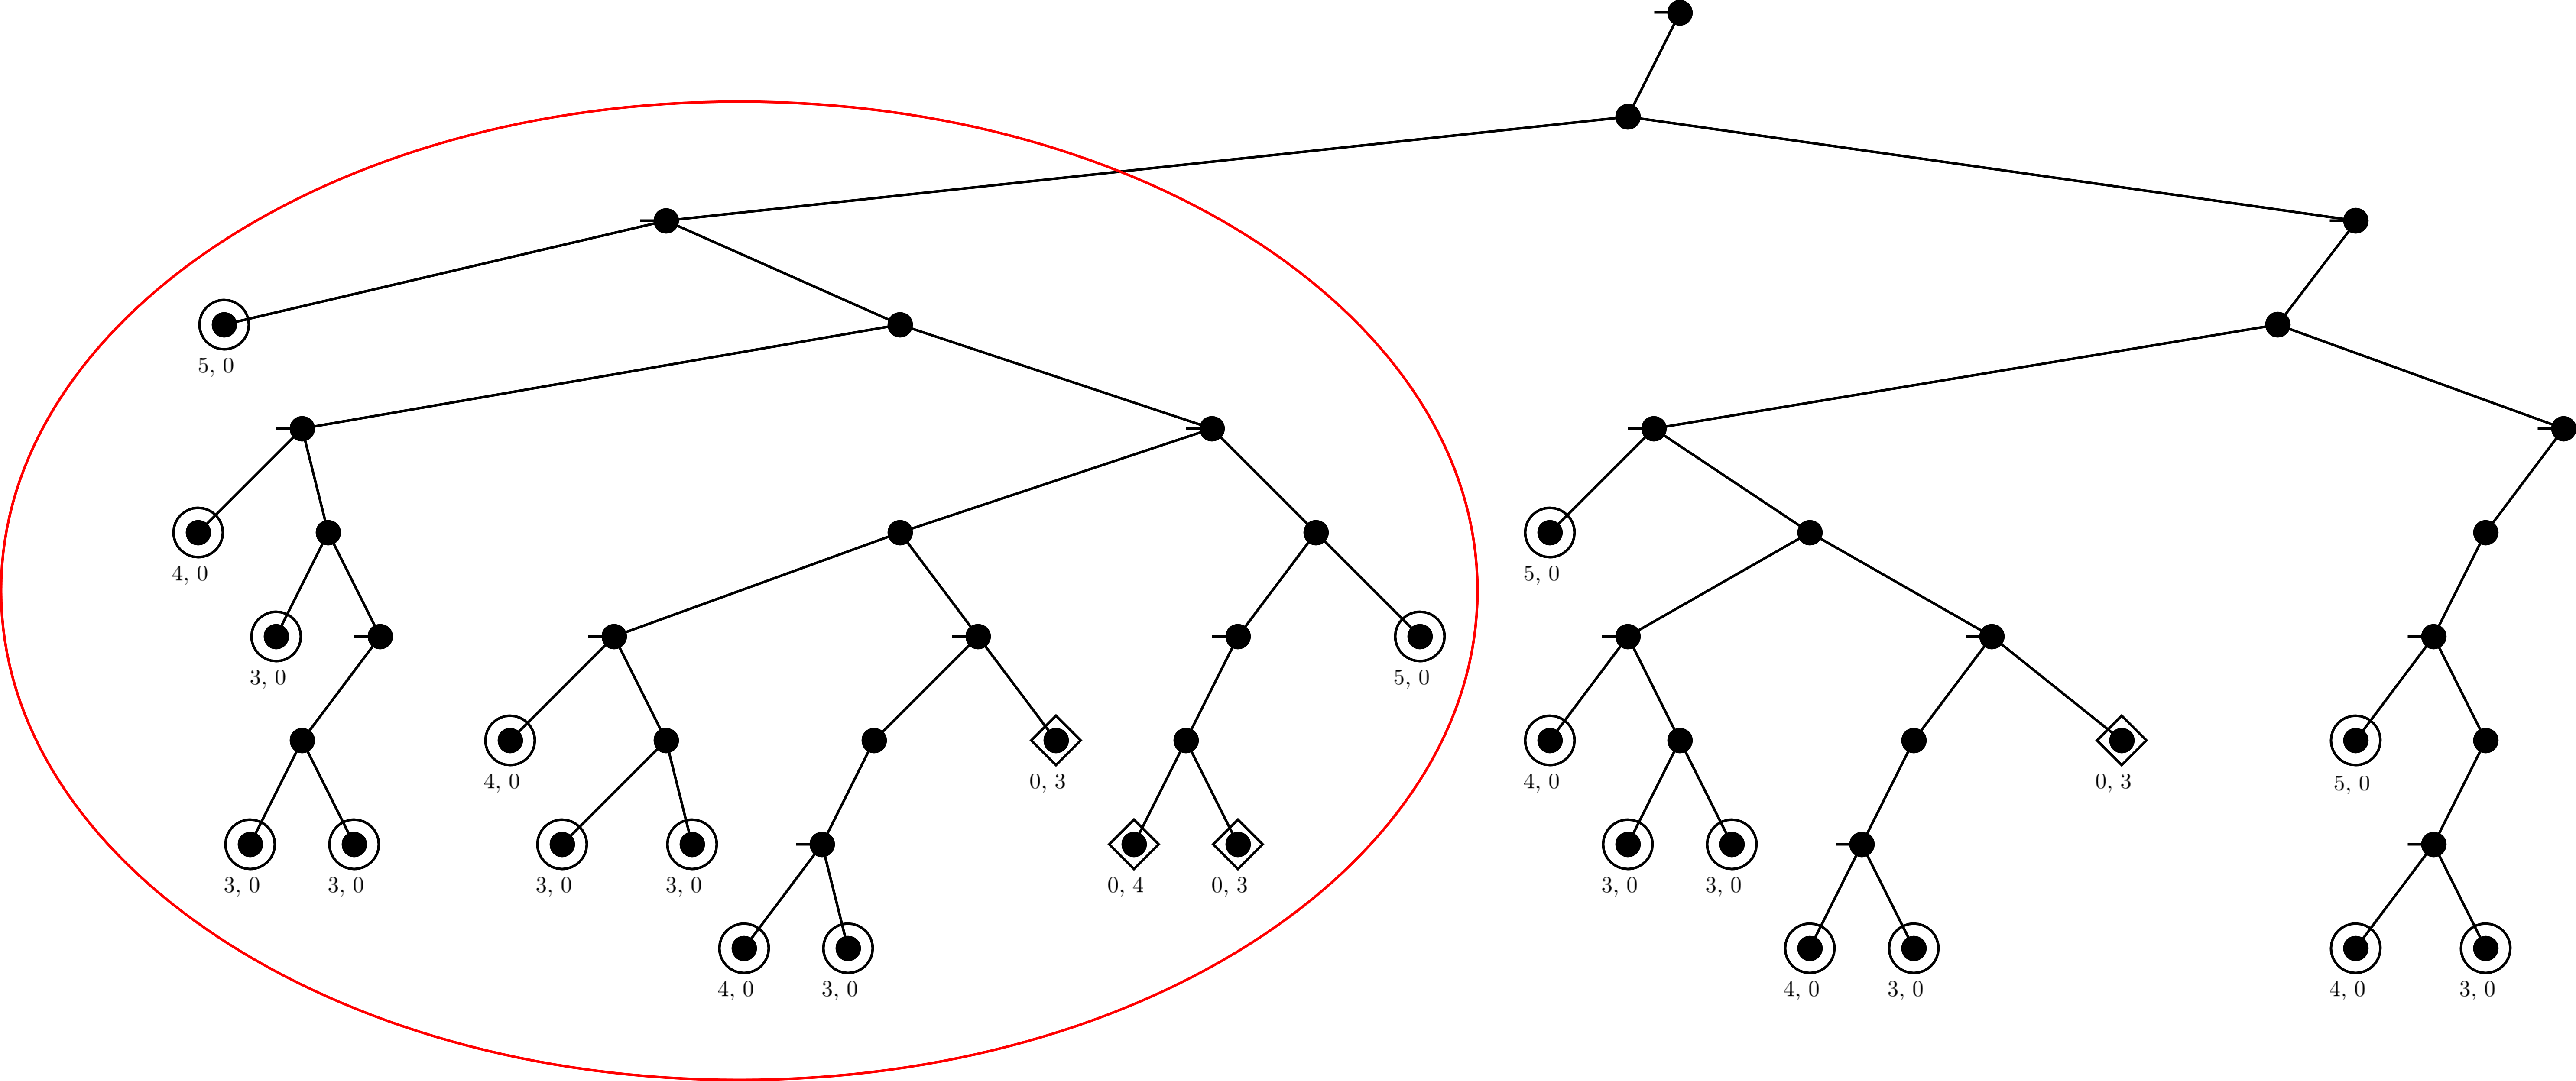
\includegraphics[width=15cm]{figures/Backwards0.png}
  \caption{The extensive-form tree for the simplified version of the game, but with extraneous nodes removed; a node is extraneous if the player making their decision has only one possible action. The circled subtree will be the first subtree examined on recursive calls of the backwards induction algorithm.}
  \label{fig:condensedTree}
\end{figure}

For the example in Figure \ref{fig:gameTree}, we can trivially condense branches where only one action is available, taking the utility values from the leaf nodes and copying them up the tree. This produces the tree seen in Figure \ref{fig:condensedTree}. We define the utility of a player in this game as their HP at the end of the game minus the HP of their opponent. Thus, for a game with the outcome (4, 0), player 1 will have a utility of 4 and player 2 will have a utility of -4.\\

The algorithm begins at the root node of the tree. Since the root is not a leaf node, the algorithm is called on the root's children, starting with the leftmost child. The root node only has one child, since players cannot heal when their HP is maxed out. So, the backwards induction algorithm is called on the next node, which does have more than one child. To find the utility of both children, the algorithm must be recursively called on both subtrees, starting with the subtree circled in red in Figure \ref{fig:condensedTree}.\\

\begin{figure}[H]
  \centering
  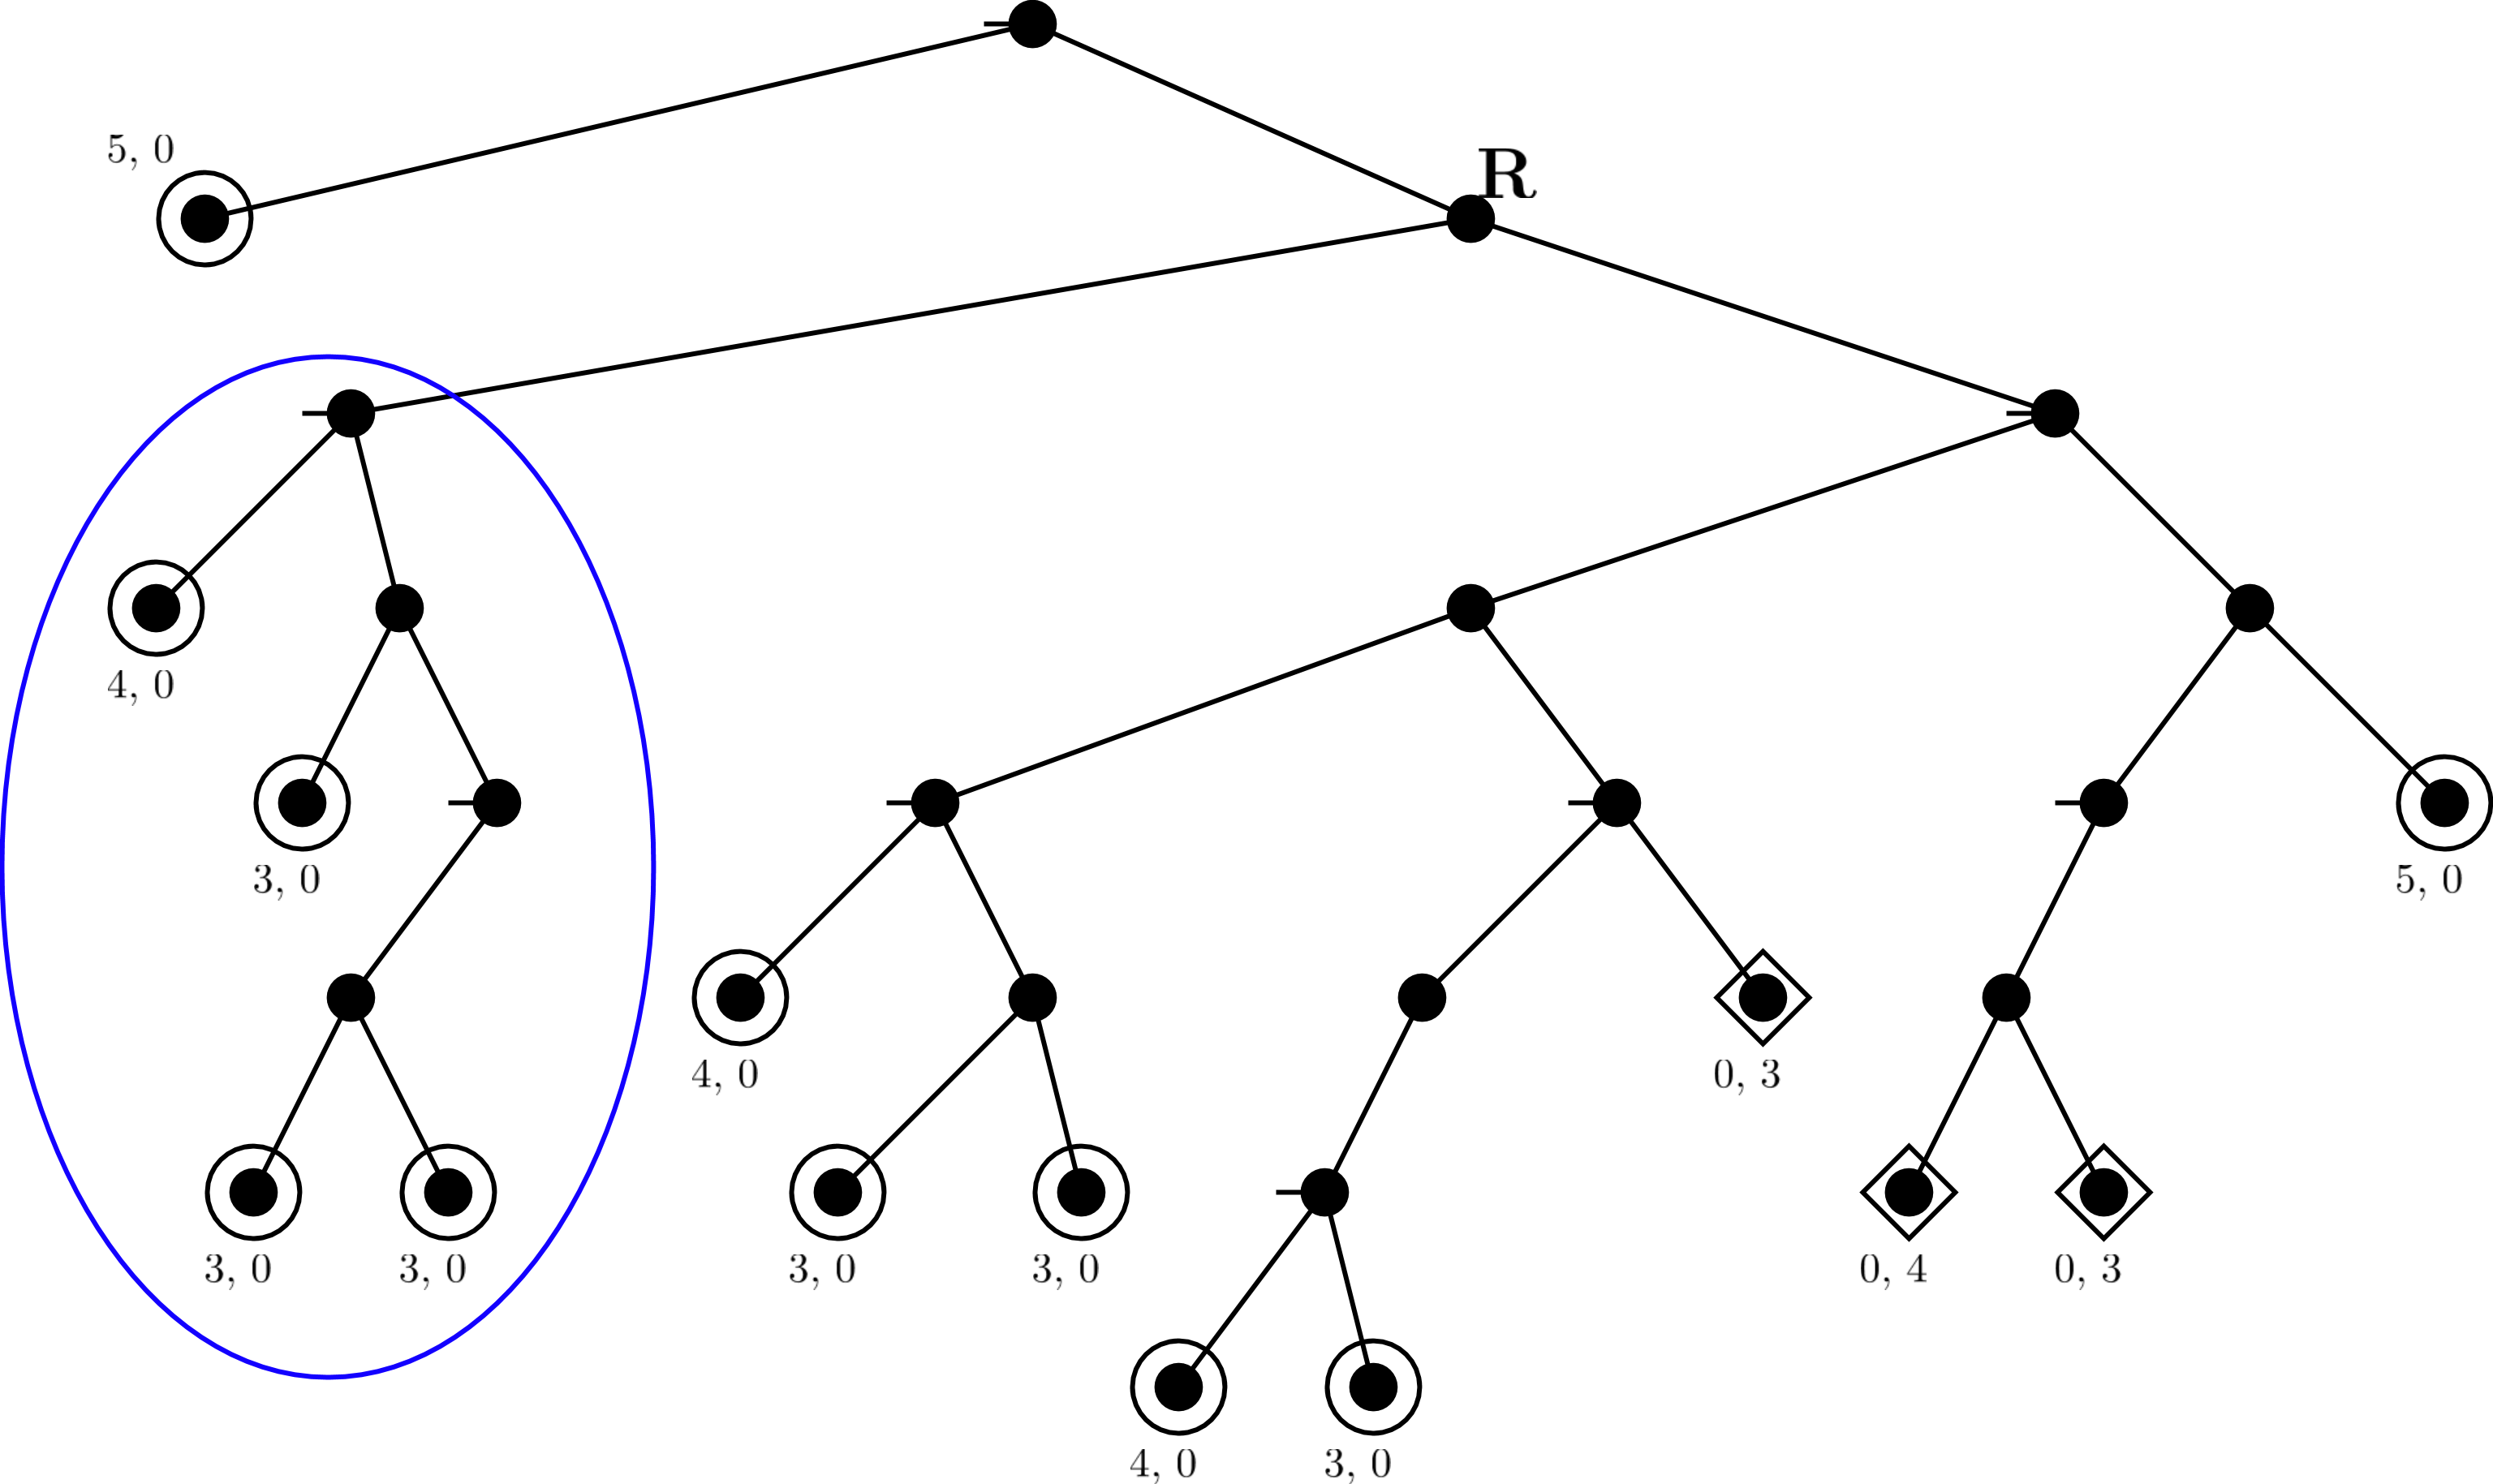
\includegraphics[width=11cm]{figures/Backwards1.png}
  \caption{The tree examined by the backwards induction algorithm after recursing to the circled subtree in Figure \ref{fig:condensedTree}.}
  \label{fig:backwards1}
\end{figure}
Examining the root of the subtree in Figure \ref{fig:backwards1}, we find that the left child of the root is a leaf node. Thus, since the root is a decision node for player 1, the utility of this entire subtree will be the maximum utility for player 1 between the leaf node (5, 0) and the utility of the right child, which is its own subtree. Once again, the backwards induction algorithm is called recursively, this time on the subtree with root $R$. On the recursive call, the left child of $R$ is the subtree circled in blue.\\

\begin{figure}[H]
  \centering
  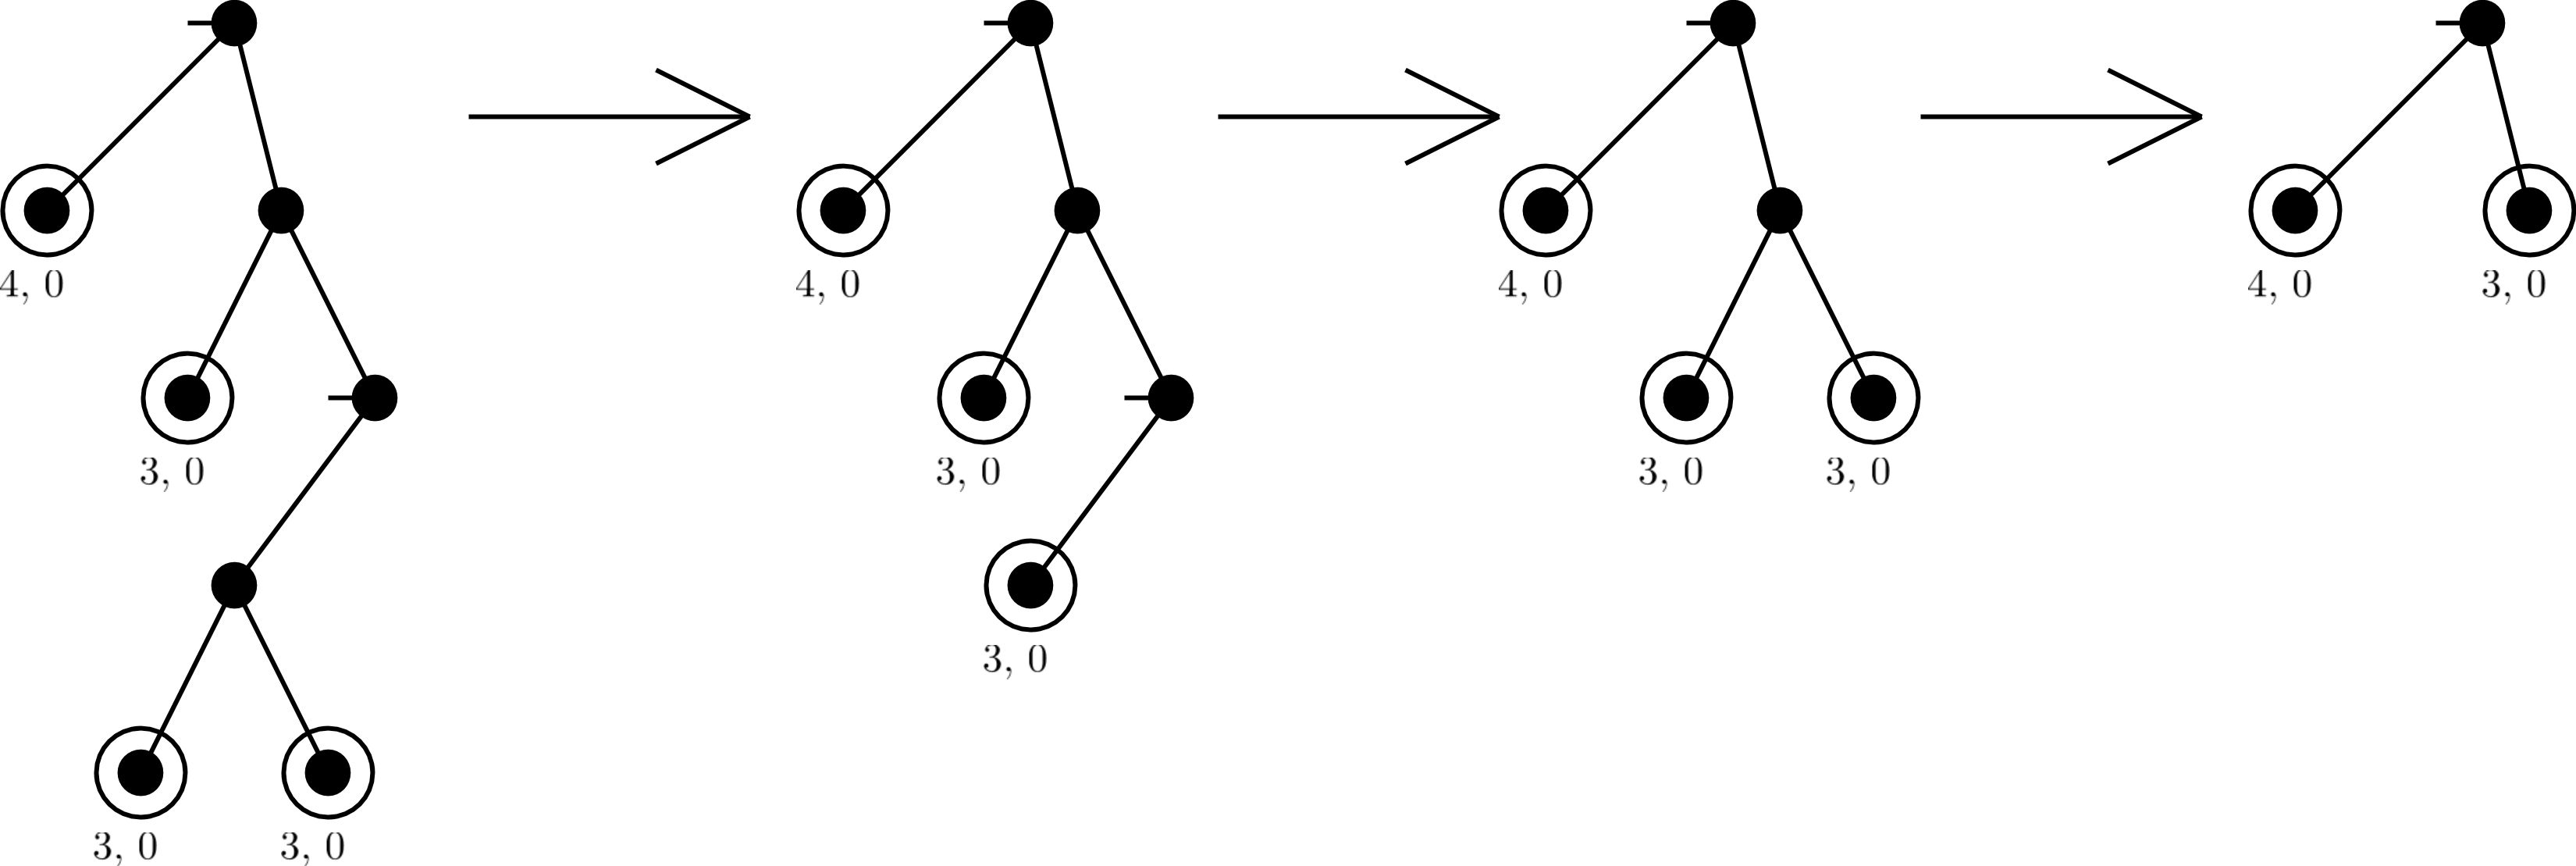
\includegraphics[width=12cm]{figures/Backwards2.png}
  \caption{The steps taken by the backwards induction algorithm after reaching the circled subtree in Figure \ref{fig:backwards1}}
  \label{fig:backwards2}
\end{figure}
As the algorithm continues to recurse through the game tree, it will eventually reach the pair of leaf nodes at the bottom of the leftmost tree in Figure \ref{fig:backwards2}. The preceding decision node is a choice for player 2, so player 2 will make whichever choice gives them more utility. In this example, both leaf nodes provide player 2 with -3 utility, so the utility of the decision node is (3, 0). This utility value is moved up the tree to the next decision node, as shown in Figure \ref{fig:backwards2}. These steps continue up the subtree. The next decision node again has a tie between (3, 0) and (3, 0), but the root of the subtree has a choice between (3, 0) and (4, 0). Since the root of this subtree is a decision node for player 1, that player will prefer to attack and reach the (4, 0) leaf node for 4 utility. Thus, the utility of the circled subtree in Figure \ref{fig:backwards1} is (4, 0).\\

\textbf{To be continued...}

\subsubsection{Analysis}
In this limited model, it is clear that healing is not a viable strategy. Since players can only attack or heal, choosing to heal will either have no affect on utility or a negative affect on utility. If one player heals and their opponent also heals, then the overall change in . The HP recovered by one player is not enough to offset the damage dealt by their opponent. At the most, choosing to heal only delays the inevitable.\\

In the four paths where player 2 won, there is a node where player 1 chose to heal from 9 HP to 10 HP. Since the normal amount of HP recovered by healing is 4 HP, we can see that player 1 is wasting potential HP by using one of their turns to heal when their HP is already close to the HP cap. We may infer that, in games with larger HP caps, the same effects would appear. It is much more useful for a player to heal when their HP is closer to zero.\\

Now that some patterns in the game are identified, we expand the game and build a prototype using Python and the pygame library.

\section{Game Engine}
Python was chosen as the development language for this game. Python is an extremely portable language: anyone with Python installed can run the code. Python also has a robust library for two-dimensional games called pygame, which was essential in creating this game. Specifically, Python 3 was used for better compatibility with the pygame library and for the copy() function for arrays.

\subsection{The pygame Library}
The pygame library provides a number of Python functions that are useful in creating a two-dimensional video game. The library was originally created in 2001 to combine Python with SDL (Simple DirectMedia Layer), a library of multimedia controls written for C \cite{shinners}. pygame can utilize a variety of different graphics libraries, including OpenGL, DirectX, the Linux frame buffer, and an ASCII art backend \cite{shinners}. The pygame library is supported by numerous operating systems, and the core functions of pygame use highly optimized C or assembly code.\\

At the top level, pygame controls the initialization and exiting of its various modules, particularly the pygame.display module which renders the game. pygame features two functions to update a display window, pygame.display.flip() and pygame.display.update(). display.flip() works with two separate arrays, containing the pixel data for the window in which the game operates. One array is displayed on the screen, while the other array is used to record changes made to the on-screen image. Once all changes are made, display.flip() swaps these arrays, or ``buffers,'' by copying all the data from one array into the other. The buffer that recorded changes is now displayed on-screen, while the buffer that was displayed can now be used to record further changes. display.update() is an optimized version of flip() that takes as an argument a rectangle or a sequence of rectangles. These rectangles correspond to the areas of the display that need to be updated. For instance, passing the coordinates of a rectangle over a game's scoreboard only updates the scoreboard. With this function, large sections of the pixel array do not need to be copied from one buffer to another, speeding up the rendering process.\\

The two main objects in pygame are the Surface object and the sprite object. Surfaces can be changed with pygame to alter various attributes. For instance, the alpha value, or the transparency of the surface, can be changed with set\_alpha(). The individual color values can be converted to integers and vice versa with the map\_rgb() and unmap\_rgb() functions, respectively. This allows for pygame to store colors as a single number, rather than a tuple of integers. Surfaces are mostly used to load image files and to create backgrounds for the game. Sprites, on the other hand, are used for the actual in-game objects, such as enemies, player characters, and projectiles. Sprites can be stored in a Group object, that can be used to separate sprites by different purposes. Each sprite draws its image to a Surface, provided that it has a Surface.image and Surface.rect attribute.\\

Once a sprite or surface is created with an image, pygame can also perform graphical transformations on that image. The pygame.transform module has functions to flip, rotate, and scale an image. Another pygame feature is the ability to do collision detection on sprites and rectangles.\\

For the actual gameplay of a pygame program, there are also modules for joystick, mouse, and keyboard controls. A sound mixer module allows audio tracks to be played in the game, and the pygame.time module can be used to control the framerate of the game.

\subsection{Gameplay Design}
For the expanded version of the game, several things were changed from the game in Figure \ref{fig:gameTree}. Two additional choices were added: Parry and Strong Attack. With Parry, the player enters a guarded stance until their next turn; this player will be referred to as the defending player. If, before their next turn, their opponent attacks them, the defending player counter-attacks. The defending player loses no HP, and the player who attacked them loses 3 HP from the counter-attack. A Strong Attack does more damage than a regular attack (7 HP vs 5 HP), but has a chance to miss the opponent completely and do no damage. Additionally, a Strong Attack is unaffected by Parry; if a player is Parrying and their opponent uses a strong attack, the parry is unsuccessful and the defending player suffers 7 HP of damage.

The two players in the game begin with 25 HP each, and are able to heal twice per game. These values are stored in a PlayerAvatar class. This class also stores the type of AI used for the computer player. The class has a helper function, which is called from within the main game loop. This helper function checks which AI model is used, then calls that model's respective function.\\

Six different AI models were created. In all models, the AI checks to see if any healing turns remain; if not, the AI defaults to a normal attack. Three of the models rely on a random number generator.\\

\begin{figure}[H]
  \centering
  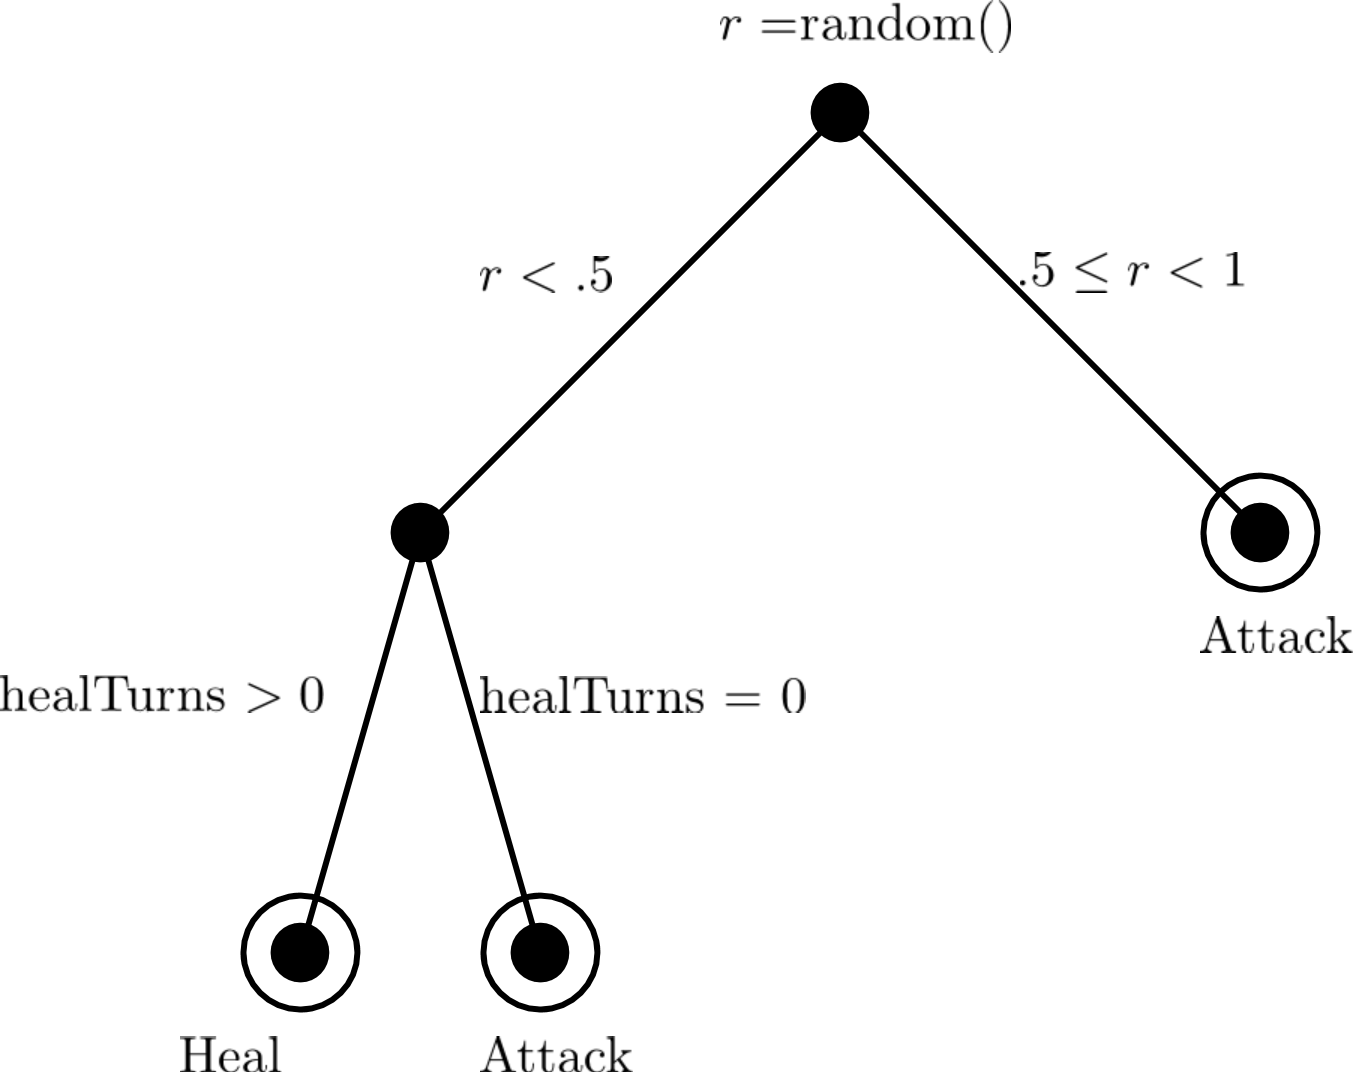
\includegraphics[width=7cm]{figures/AILimitedRandom.png}
  \caption{The decision tree for the limitedRandomAI() function.}
  \label{fig:AI1}
\end{figure}

The first AI model, the limitedRandomAI() function, chooses randomly to attack or heal with a 50/50 chance of either, but will attack instead if the AI has already healed itself twice. This is shown by the decision tree in Figure \ref{fig:AI1}. The variable $r$ is given a random value between 0 and 1, and the first decision in the tree is based on the value of $r$. After that, the tree has either reached a leaf node (for $r\ge .5$) or must make a second decision, this time based on the number of heal turns remaining. Given the limited success player 2 had in the original game tree in Figure \ref{fig:gameTree}, this model was not used in the final version of the game. Instead, a different model was used which could perform all four possible actions.\\

\begin{figure}[H]
  \centering
  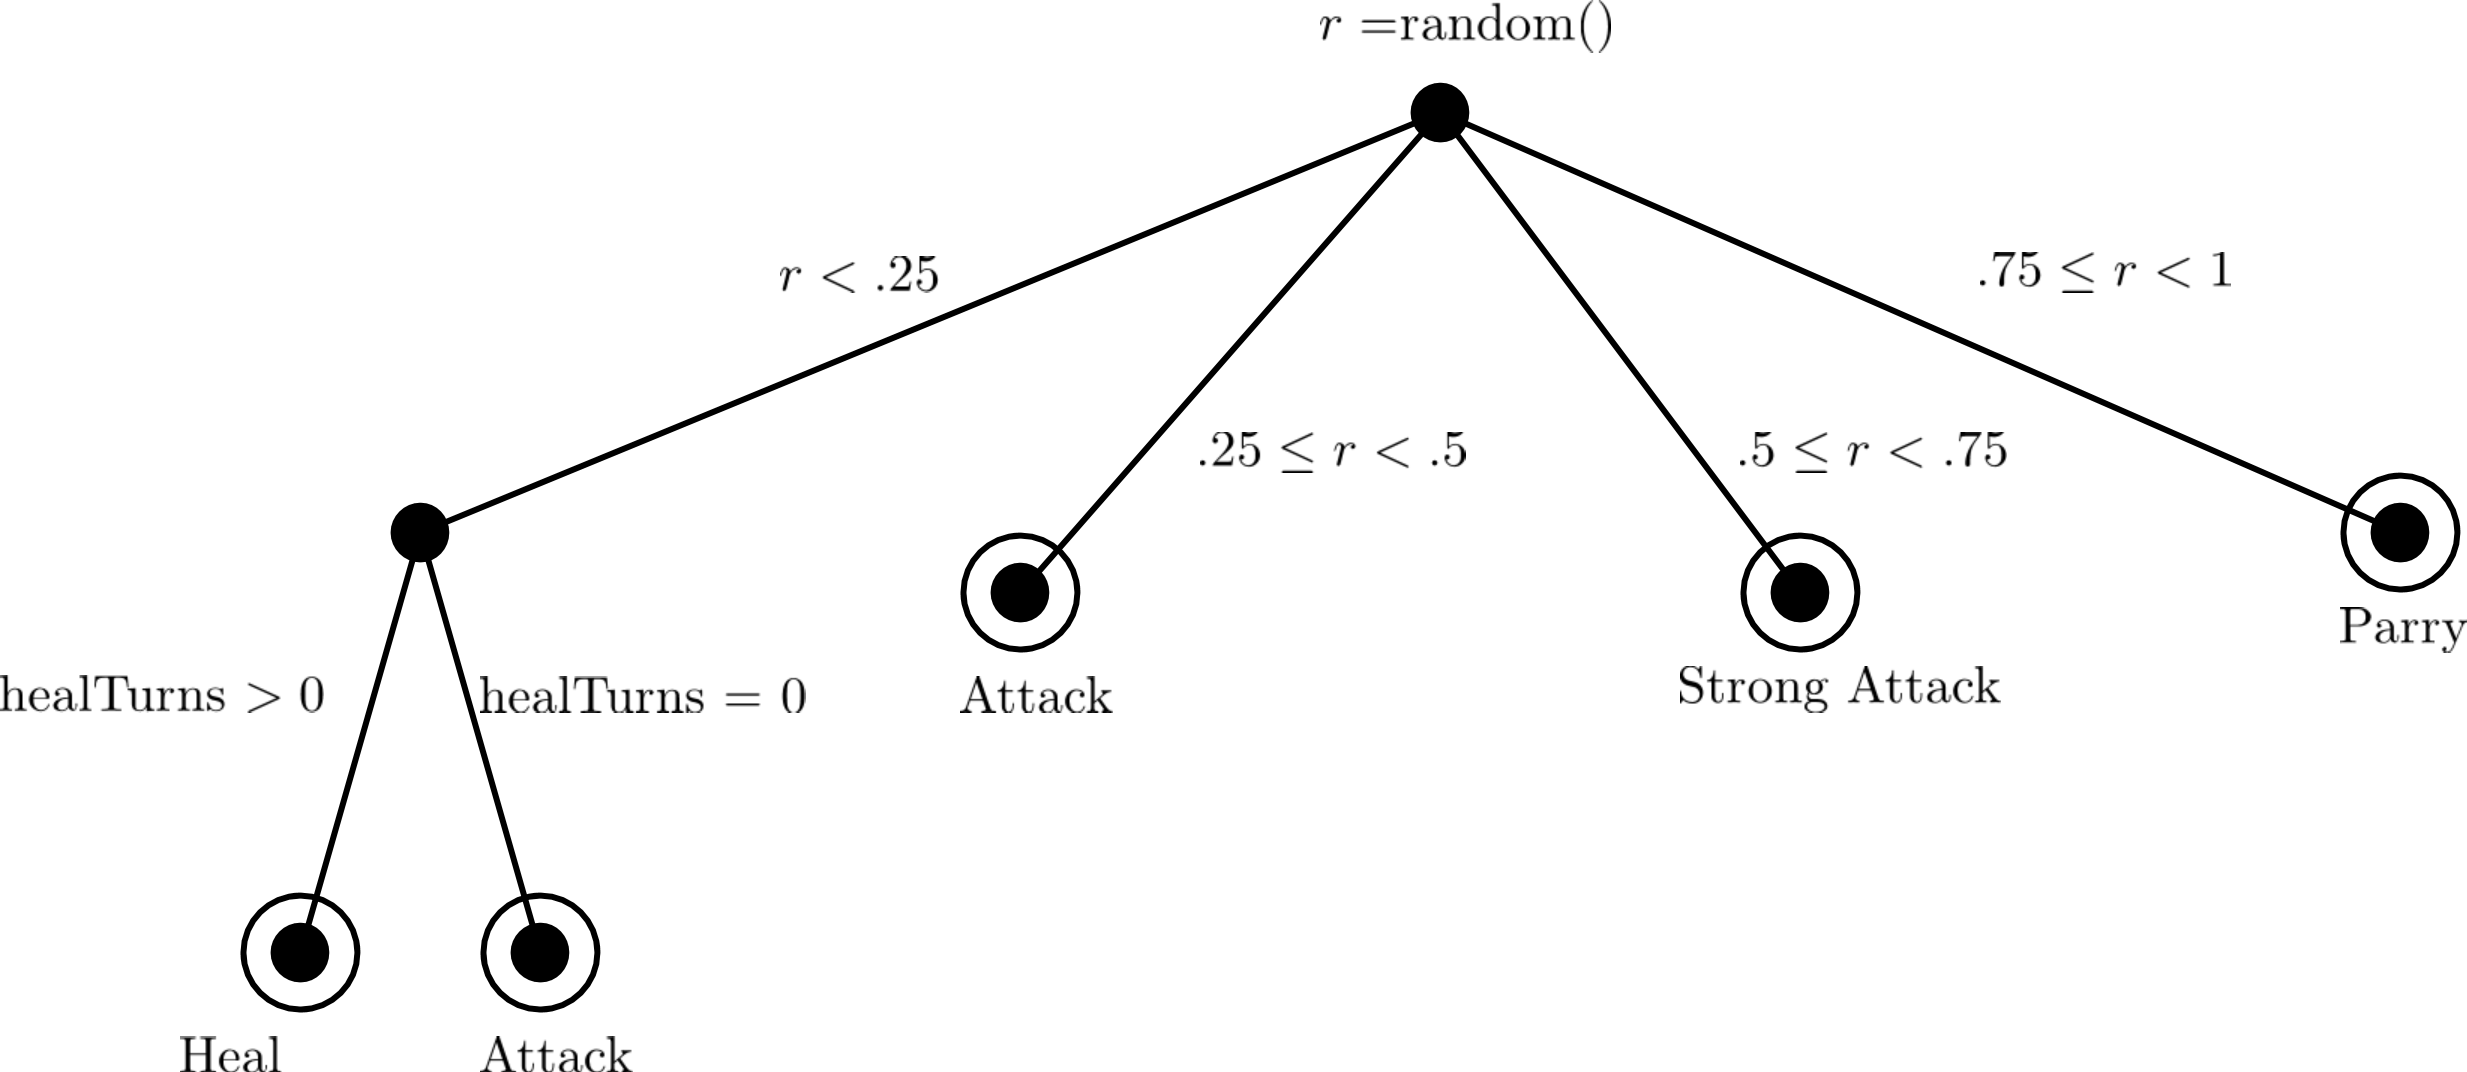
\includegraphics[width=11cm]{figures/AIRandom.png}
  \caption{The decision tree for the randomAI() function.}
  \label{fig:AI2}
\end{figure}
The second model, randomAI(), has a 25\% chance of attacking, healing, parrying, or using a strong attack. Again, Figure \ref{fig:AI2} shows that if the random number generator chooses to heal, but all healing turns have been used, the AI does a normal attack instead. This choice was made to effect a kind of desperation to fights: when an opponent no longer can heal themselves, they become more offensive to try and win the battle. This kind of behavior - where the AI changes their strategy after all healing turns have been spent - is incorporated into all the models.\\

\begin{figure}[H]
  \centering
  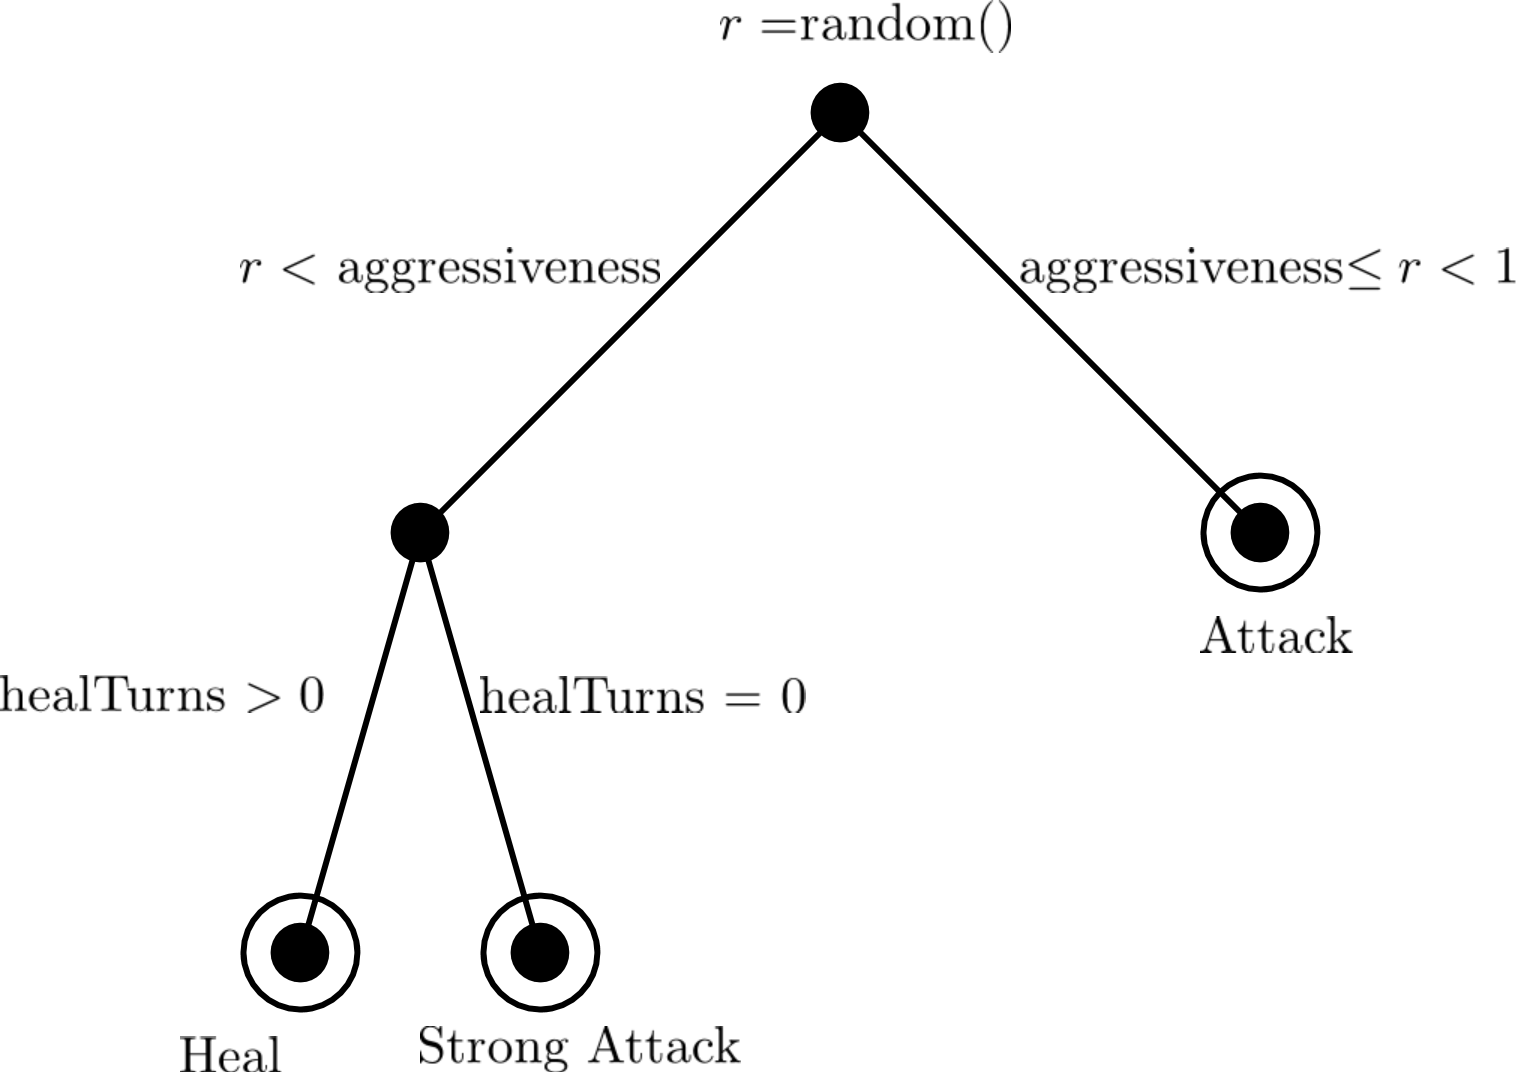
\includegraphics[width=9cm]{figures/AIAgressive.png}
  \caption{The decision tree for the aggressiveRandomAI() function.}
  \label{fig:AI3}
\end{figure}

The third model, aggressiveRandomAI(), is the final model which uses a random number generator. For this model, there is an additional variable given to the AI player, the aggressiveness stat. Rather than evenly splitting up actions 50-50, the choice between attacking and healing is split along this aggressiveness, which is a real number between 0 and 1. For this thesis, the aggressiveness was set to .25, leading to an AI which attacked 75\% of the time and healed 25\% of the time. As can be seen in the decision tree in Figure \ref{fig:AI3}, the AI uses strong attacks when the random number $r$ is below the aggressiveness stat and the two allotted heal turns are expended.

\begin{figure}[H]
  \centering
  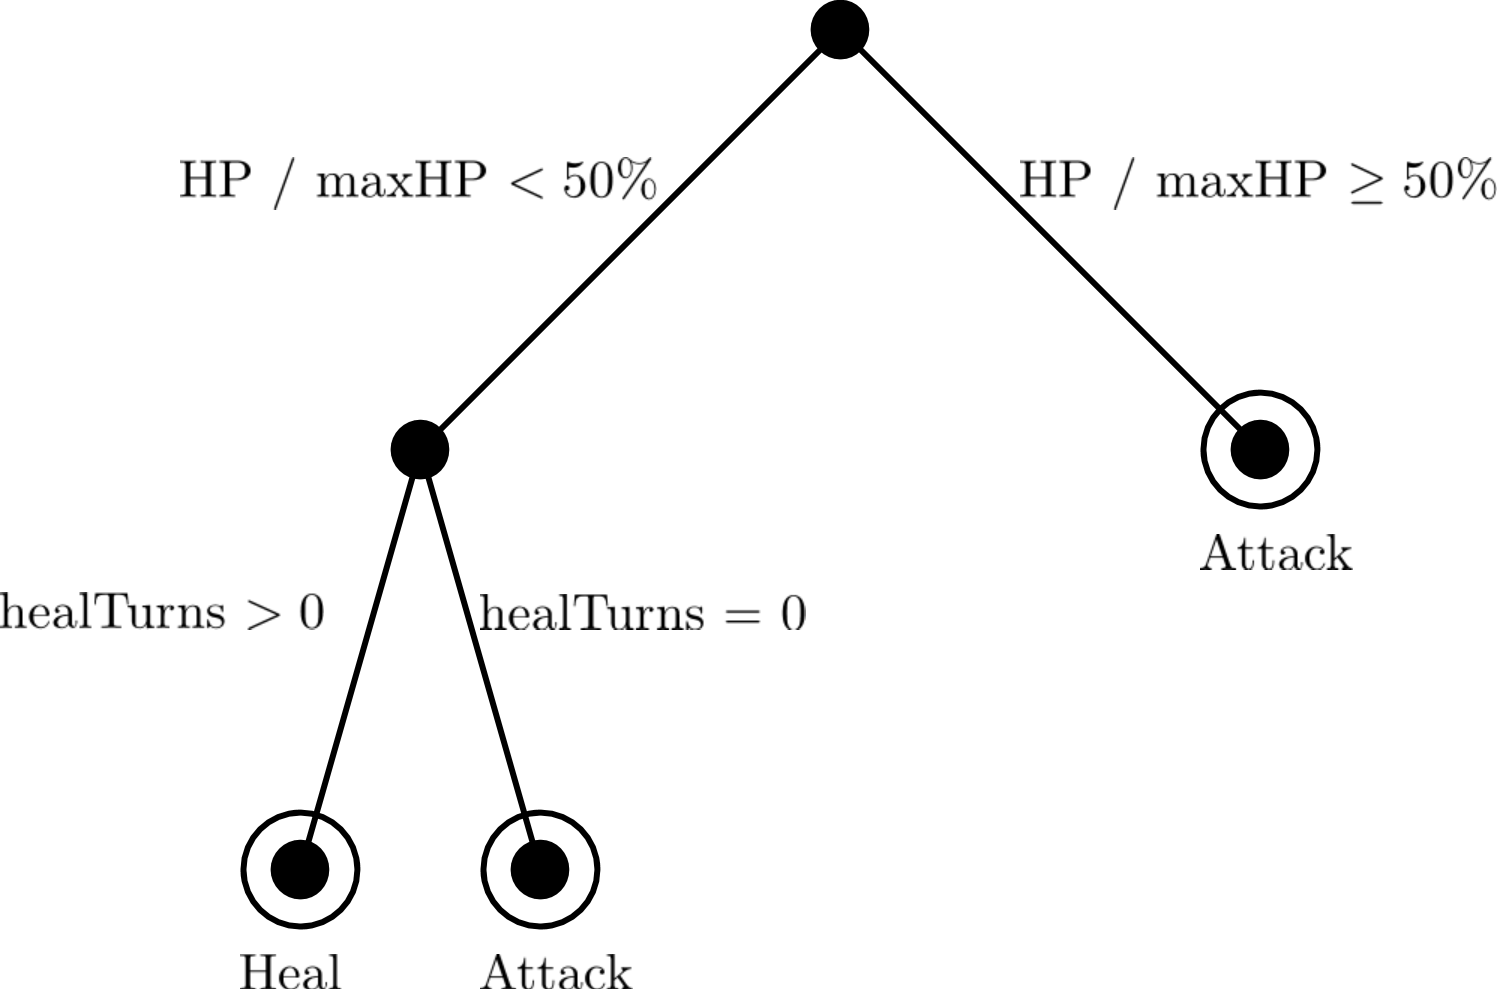
\includegraphics[width=9cm]{figures/AI50Percent.png}
  \caption{The decision tree for the fiftyPercentAI() function.}
  \label{fig:AI4}
\end{figure}

In the fourth model, fiftyPercentAI(), the AI only heals when its health falls below 50\% of its maximum. Thus, the AI only heals when it is close to death, as opposed to the random AI models which could potentially waste their heals at the start of a game. As shown in Figure \ref{fig:AI4}, this AI only uses normal attacks and heals; it does not do any parrying or strong attacks. Thus, it has the most in common with the limitedRandomAI() function with regards to possible actions. However, by saving heals until later in the game, this model has some semblance of intelligence, whereas the limitedRandomAI() does not.

\begin{figure}[H]
  \centering
  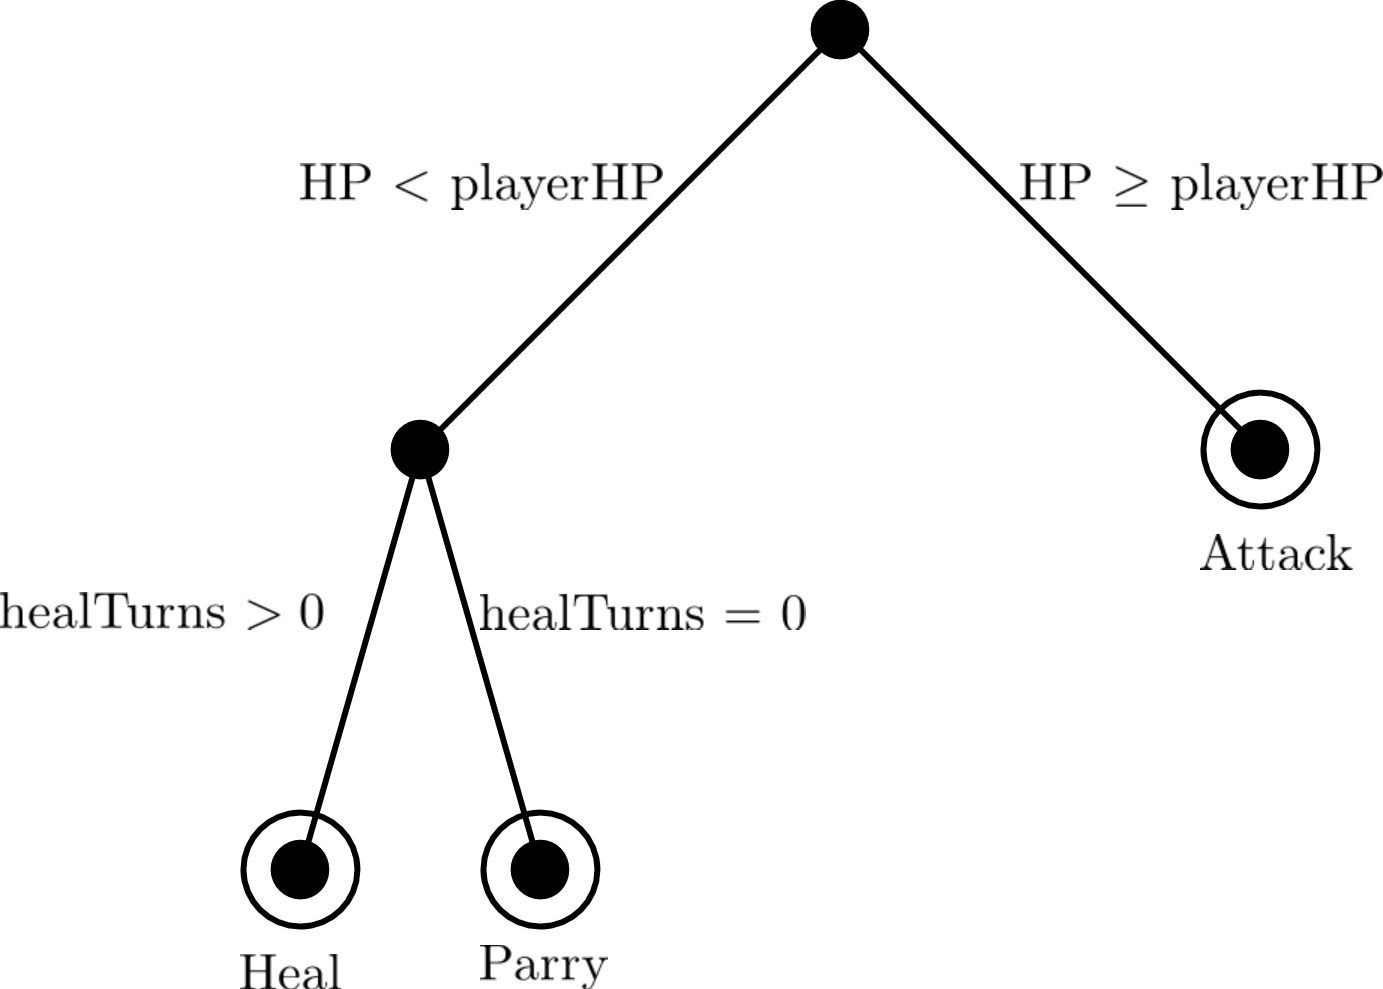
\includegraphics[width=8cm]{figures/AIComparative.png}
  \caption{The decision tree for the comparativeAI() function.}
  \label{fig:AI5}
\end{figure}

The fifth model uses similar tactics as fourth, but instead of using 50\% as the threshold, the AI heals whenever its HP drops below the player's HP, as seen in Figure \ref{fig:AI5}. Additionally, when the AI has expended all its healing turns and its HP falls below the player's HP, the AI uses a parry instead of an attack. Over the course of a game, the AI will defend itself, relying on counter-attacks to weaken the player before making attacks of its own.

\begin{figure}[H]
  \centering
  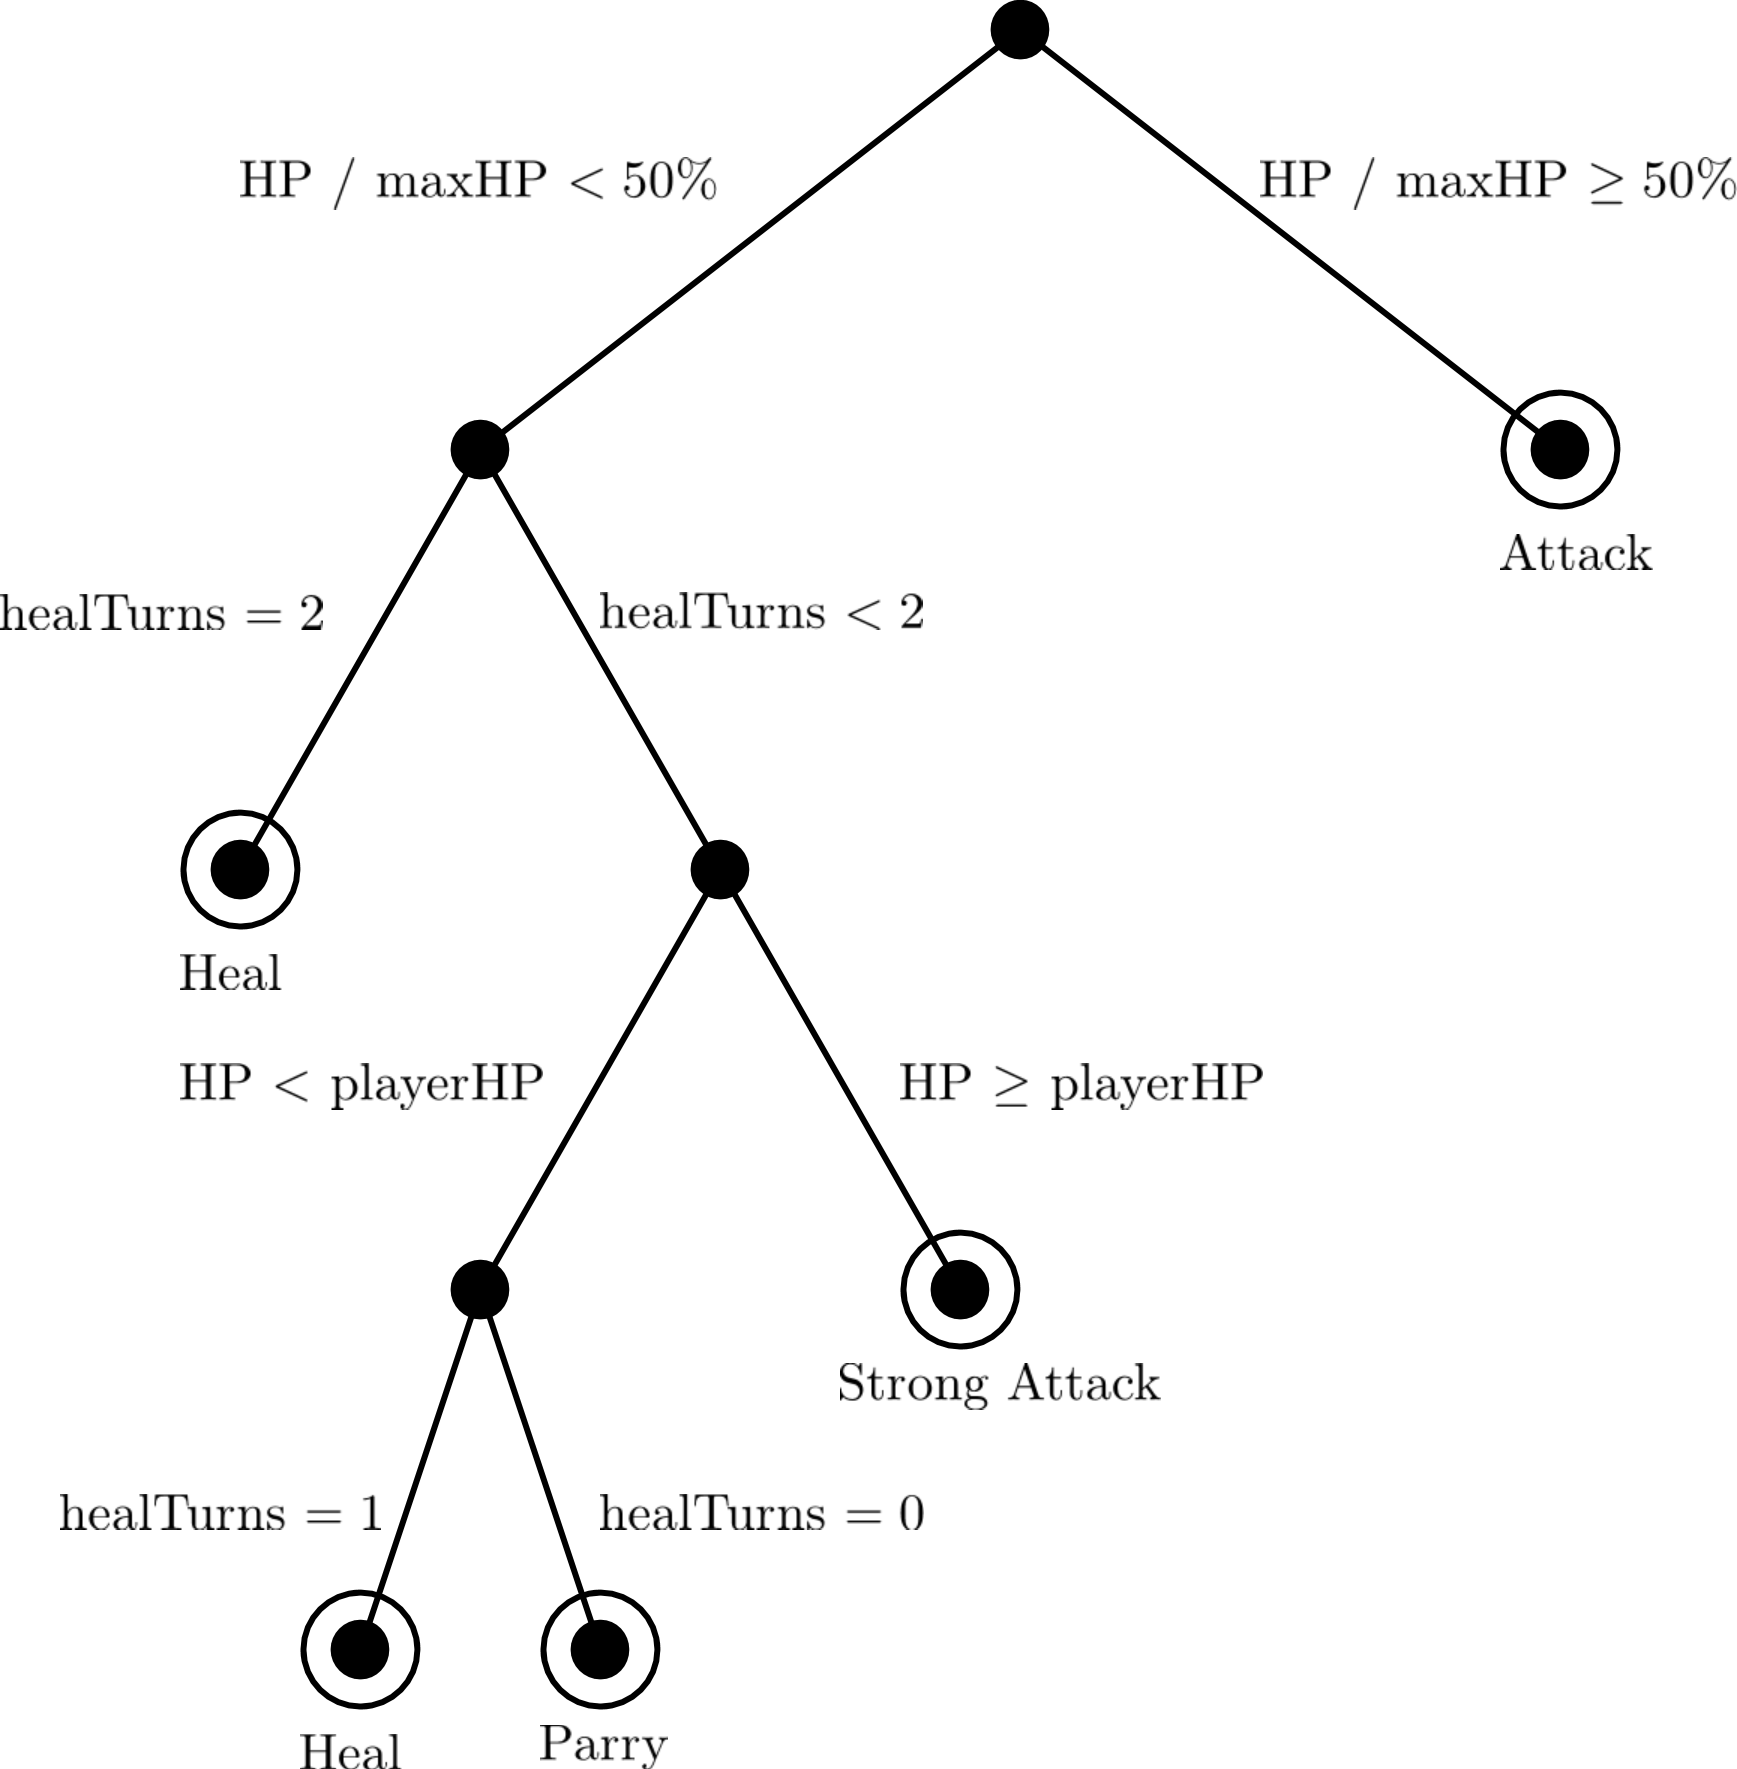
\includegraphics[width=10cm]{figures/AIScaling.png}
  \caption{The decision tree for the scalingDifficulty() function.}
  \label{fig:AI6}
\end{figure}

Finally, the scalingDifficulty() model in Figure \ref{fig:AI6} is a loose combination of the fiftyPercentAI() and comparativeAI() functions. As in \ref{fig:AI4}, the AI performs a normal attack whenever the AI's HP is above 50\% of its maximum. In this model, the two available healing turns are used in different circumstances. The first healing turn is used when the AI drops below 50\% HP for the first time. If their HP drops below 50\% after this first healing turn, the AI becomes more strategic. If the AI is below 50\% but still has a greater HP value than the player, then the AI will use strong attacks. However, if the AI is both below 50\% and below the player's HP, then it will use its second healing turn if available and parry if no healing turns remain.\\

\subsection{Visual Design}
The visual design of the game was left fairly simple, to avoid distracting players from the strategic elements of the game. Icons for the player character and enemy opponents were created in the GNU Image Manipulation Program (GIMP), then imported as pygame sprites using the pygame.image.load() function. Since these sprites had a transparency component, the function convert\_alpha() was also used to preserve this transparency in pygame.\\

\begin{figure}[H]
  \centering
  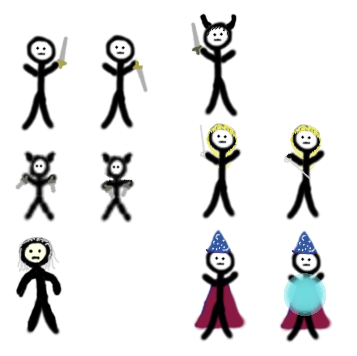
\includegraphics[width=9cm]{sprites/SpriteSheet.png}
  \caption{The set of sprites used for the characters in \textit{Cave Escape}. Clockwise from top left, the characters are the player character, an orc, an elf, a magician, a troll, and a goblin.}
  \label{fig:SpriteSheet}
\end{figure}

\begin{figure}[H]
  \centering
  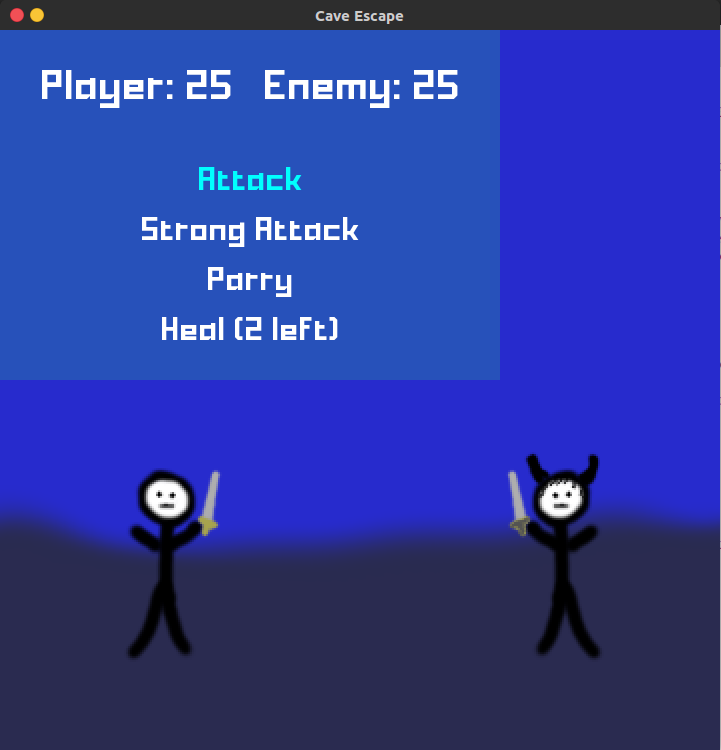
\includegraphics[width=7cm]{figures/In-Game.png}
  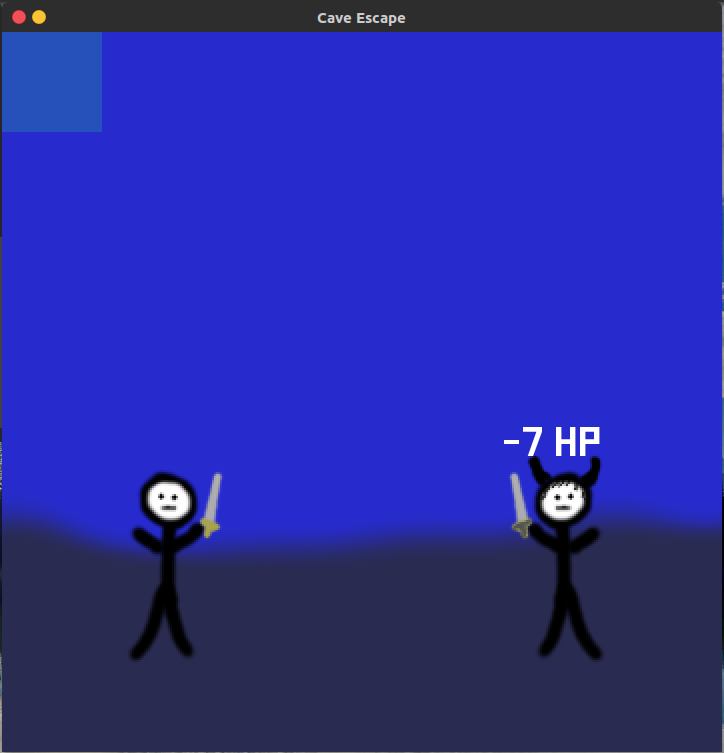
\includegraphics[width=7cm]{figures/In-Game2.png}
  \caption{In-game screenshots from \textit{Cave Escape}. The player character is situated on the left, while the opponent - an orc - is stationed on the right. The HP values of both player and AI are listed at the top of the screen. In the left image, the player is able to select their next move from the list of options. In the right image, the player has selected ``Strong Attack'' and the resulting damage is shown above the enemy's head.}
  \label{fig:ingame}
\end{figure}

An individual sprite was created for the player character and each of the five AI models, as shown in Figure \ref{fig:SpriteSheet}. These sprites are overlain on a bluish-purple background, symbolizing the cave interior. The list of possible actions is also shown on-screen, positioned above the player character as in Figure \ref{fig:ingame}. Next to the ``Heal'' option, the number of remaining healing turns is listed and updated after each turn. The HP of both players is also updated after every turn. Additionally, after players select an action, the resulting change in HP is shown above the head of the respective target. The right image in Figure \ref{fig:ingame} shows that the orc was hit by a strong attack made by the player, and took 7 points of damage.\\

Each non-player character has a respective AI model which it uses. The goblin uses the randomAI() function in Figure \ref{fig:AI2}, where all actions have a 25\% chance of being chosen. The troll uses aggressiveRandomAI(), as seen in Figure \ref{fig:AI3}. This character attacks more often that it heals, and can perform strong attacks after both healing turns are spent. The orc uses the fiftyPercentAI() function from Figure \ref{fig:AI4}. The elf is assigned to the comparativeAI() function seen in Figure \ref{fig:AI5}, and finally the magician uses the scalingDifficulty() function from Figure \ref{fig:AI6}.

\begin{figure}[H]
  \centering
  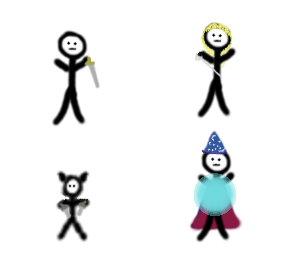
\includegraphics[width=9cm]{sprites/ParrySheet.png}
  \caption{The set of sprites used when a character is parrying. Clockwise from top left, the characters able to parry are the player character, an elf, a magician, and a goblin.}
  \label{fig:ParrySheet}
\end{figure}

In addition to the default sprites shown in Figure \ref{fig:SpriteSheet}, characters have a second sprite for when they are parrying. The Troll and Orc characters are unable to parry, so only four of these sprites were created. These variants are shown in Figure \ref{fig:ParrySheet}: the player character, the elf, the magician, and the goblin all have parry sprites.\\

At runtime, the game starts at a menu screen, where the five enemy characters are listed. When the HP of either the player or the AI falls to 0 or lower, the round ends. A final screen is shown to either celebrate the player's victory or lament their failure.

\section{Playtesting and Survey}
To test the effectiveness of these AI models, a group of participants were surveyed to play the various models. Each participant played five rounds against one of the models. The program collects data on wins and losses, as well as the sequence of actions taken by both the human player and the AI opponent. In addition to this game data, a short survey was given to each participant. Subjects were asked to answer the first three questions before playing the game. These questions asked participants to rate, on a scale of 1 to 5, their interests in video games, strategic board games, and RPGs, respectively. A score of 1 indicated little or no interest, while a score of 5 indicated a strong interest. After the three questions, participants were given a short description of the game, including the possible actions that players could take in the game. After the participant completed the five rounds, they were asked three more questions. These questions asked them to rate, on a scale of 1 to 5, how fun they found the game, how understandable the controls were, and how aggressive or passive their playstyle. 1 indicates a rating of not fun, that the controls were not understandable at all, and that the player used a very passive playstyle, respectively. A 5 rating indicated that the participant had a lot of fun, that the controls were very understandable, and that their playstyle was very aggressive, respectively.